
\subsection{Results by Fields of Study}
The varying preferences of female students across different fields of study  in post-secondary schooling decisions can be illuminated by three key factors: social dynamics, role models and mentors, and perceived stereotypes and bias.

In areas such as Economics, Business, Social Sciences/Humanities, Education Sciences, Health Sciences (except Medicine), Medicine, and Law, female students exhibit a higher preference  (See more details on preferred majors for female students in Subsection \ref{subsec:prefered_female}). This preference may be influenced by the presence of supportive social dynamics within these fields, where female students feel a sense of belonging and encouragement. Additionally, the availability of visible role models and mentors in these disciplines could inspire female students to pursue further studies.

Conversely, in fields such as Engineering, Architecture, Mathematics and Natural Sciences, female students exhibit a lower preference, potentially influenced by entrenched stereotypes suggesting these disciplines are more suited for males(For further details, refer to Subsection \ref{subsec:less_preferred_female}).. This bias, compounded by the competitiveness often observed in male students, tends to favor the choice of STEM-related careers, further dissuading female participation.



Interestingly, some areas such as Fine Arts and Agronomy/Veterinary-related fields demonstrate a similar level of preference between male and female students(For more insights, refer to Subsection \ref{subsec:similar_preference}). This parity suggests that in disciplines where social dynamics are more balanced, and stereotypes and biases are less pronounced, both genders may feel equally encouraged to pursue further studies.


\subsubsection{Fields of Study  Preferred by Female Students} \label{subsec:prefered_female}
In this section, we analyze the fields of study  where female students demonstrate a higher preference compared to male students.

1. \textbf{Economics, Business and  Related Majors}: The \citet{SUN2021175} estimation, depicted in the figure \ref{fig:staggered_economics_business} illustrates that the change in gender at school apparently does not significantly affect the decision to participate in careers related to administration and economics. However, it is crucial to note, as mentioned previously, that this observation only reflects the minimum diversity compositions of the new gender in the former single-gender schools. Therefore, the study depicted in Figure  \ref{fig:economics_business_related} becomes essential, as it considers several gender compositions and their relationship on career choices.
 


\begin{figure}[H]
    \centering
    \begin{subfigure}[b]{0.45\textwidth}
        \centering
        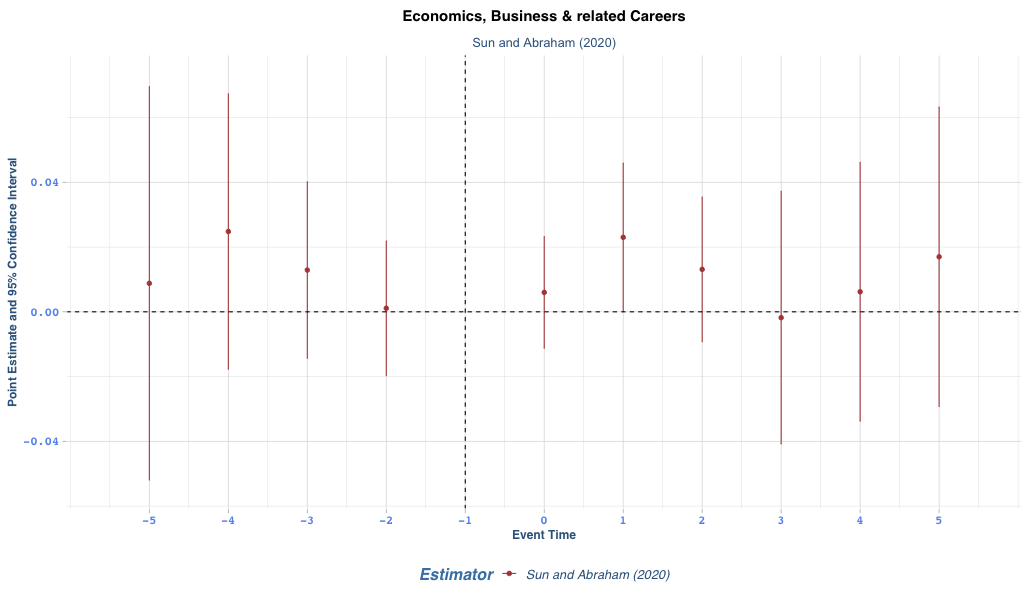
\includegraphics[width=\textwidth]{Graph/Results/stagered_ex_females_ECONOMICS_BUSINESS_RELATED.png}
        \caption{Ex female schools }
        \label{fig:staggered_females_economics_business}
    \end{subfigure}
    \hfill
    \begin{subfigure}[b]{0.45\textwidth}
        \centering
        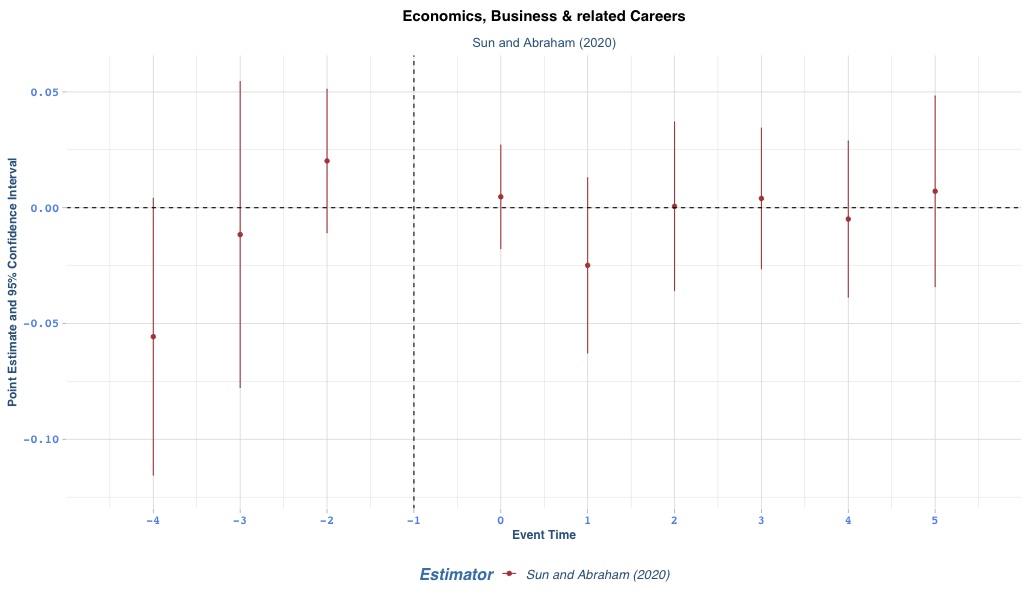
\includegraphics[width=\textwidth]{Graph/Results/stagered_ex_males_ECONOMICS_BUSINESS_RELATED.png}
        \caption{Ex male schools }
        \label{fig:staggered_males_economics_business}
    \end{subfigure}
\caption{ Changes in the Proportion of Students Choosing Economics and Business Related Majors in Schools Transitioning from Single-Sex to Coeducational}
    \label{fig:staggered_economics_business}
\end{figure}

The odds ratio for female students selecting majors in economics and business-related fields exhibits variation in response to changes in the male composition fraction within the classroom (See Figure \ref{fig:economics_business_related}).  As the proportion of male students increases, the odds ratio demonstrates fluctuation, reflecting the nuanced influence on female students' decisions regarding these majors. Higher proportions of male students in the classroom correlate with elevated odds ratios, suggesting a potential inclination among female students toward these majors in more gender-diverse environments. Notably, the analysis reveals that the odds ratio for the entire sample (12,120 students, depicted by the red line) peaks when the composition of male students in a classroom reaches approximately 29.22\%, with a substantial difference of 25 percentage points (0.64 - 0.39). This finding underscores the significant impact of classroom demographics on female students' preferences and underscores the importance of fostering gender diversity within educational settings.
 
\begin{figure}[H]
\centering
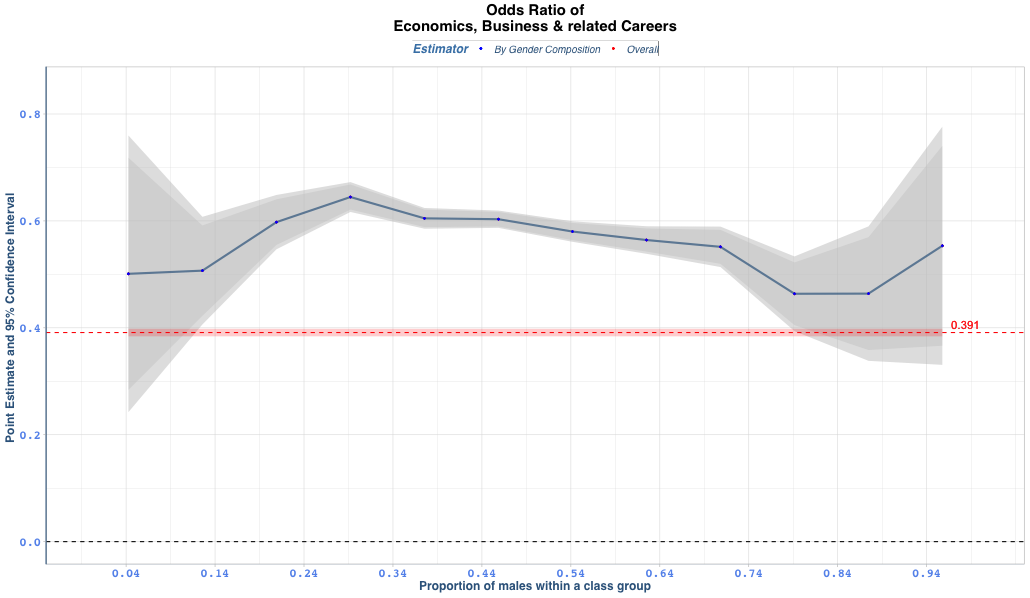
\includegraphics[width=0.8\textwidth]{Graph/Results/fe_panel_student_gender_composition_wome_in_ECONOMICS_BUSINESS_RELATED_bce.png}
\caption{Likelihood of a female student choosing economics/business-related majors}
\label{fig:economics_business_related}
\end{figure}

% Your analysis goes here


2. \textbf{Social Sciences/Humanities Majors}: The odds ratio for female students opting for majors in social sciences and humanities also varies with the male composition fraction in the classroom. Interestingly, unlike some other fields, higher proportions of male students are associated with higher odds ratios, indicating a potential preference among female students for these majors in more gender-diverse environments.

\begin{figure}[H]
    \centering
    \begin{subfigure}[b]{0.45\textwidth}
        \centering
        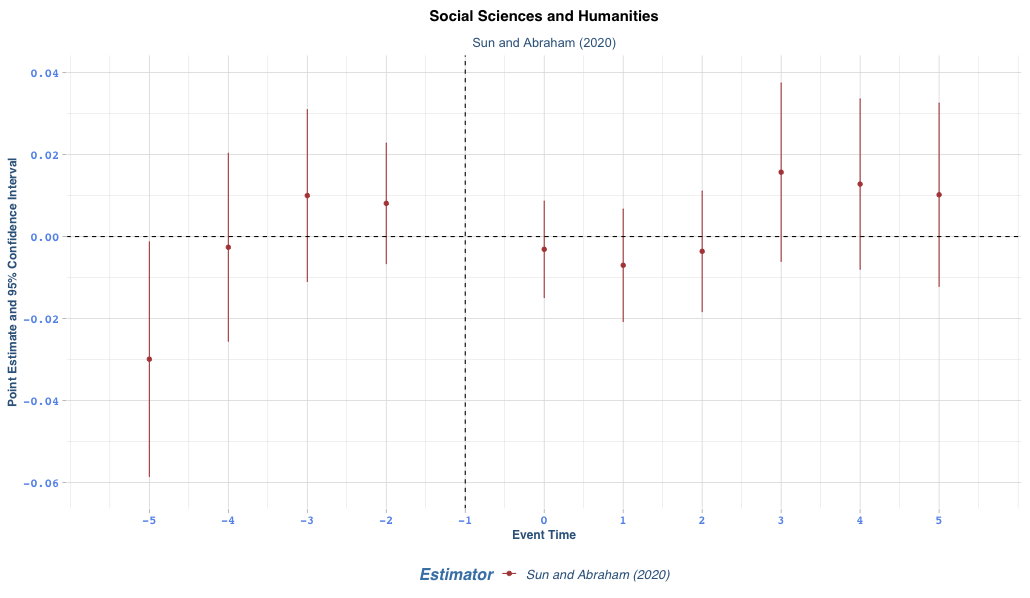
\includegraphics[width=\textwidth]{Graph/Results/stagered_ex_females_SOCIAL_SCIENCES_HUMANITIES.png}
        \caption{Ex female schools}
        \label{fig:staggered_females_social_sciences_humanities}
    \end{subfigure}
    \hfill
    \begin{subfigure}[b]{0.45\textwidth}
        \centering
        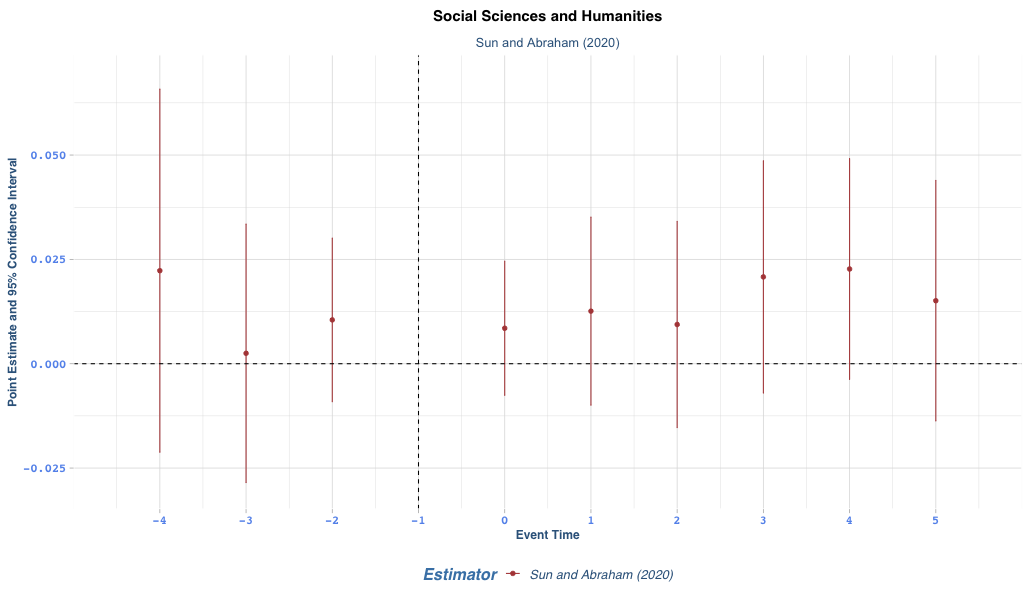
\includegraphics[width=\textwidth]{Graph/Results/stagered_ex_males_SOCIAL_SCIENCES_HUMANITIES.png}
        \caption{Ex male schools}
        \label{fig:staggered_males_social_sciences_humanities}
    \end{subfigure}
   \caption{ Changes in the Proportion of Students Choosing Social Sciences   in Schools Transitioning from Single-Sex to Coeducational}
    \label{fig:staggered_social_sciences_humanities}
\end{figure}


\begin{figure}[H]
\centering
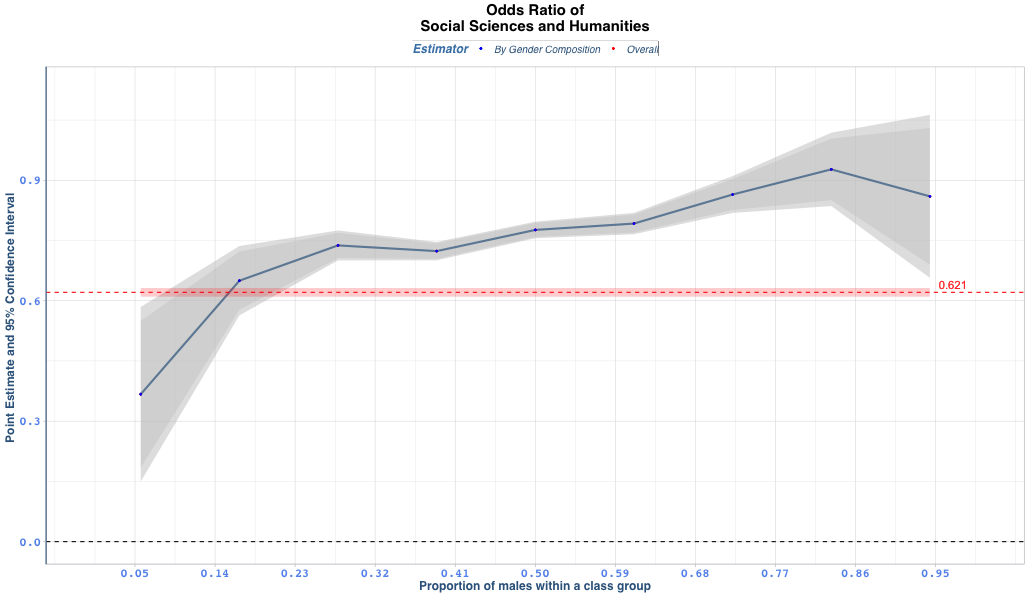
\includegraphics[width=0.8\textwidth]{Graph/Results/fe_panel_student_gender_composition_wome_in_SOCIAL_SCIENCES_HUMANITIES_bce.png}
\caption{Likelihood of a female student choosing social sciences/humanities majors}
\label{fig:social_sciences_humanities}
\end{figure}


3. \textbf{Education Sciences Majors}: The odds ratio for female students choosing majors in education sciences demonstrates variability based on the male composition fraction in the classroom. Interestingly, higher proportions of male students are associated with higher odds ratios, indicating a potential preference among female students for these majors in more gender-diverse environments.

\begin{figure}[H]
    \centering
    \begin{subfigure}[b]{0.45\textwidth}
        \centering
        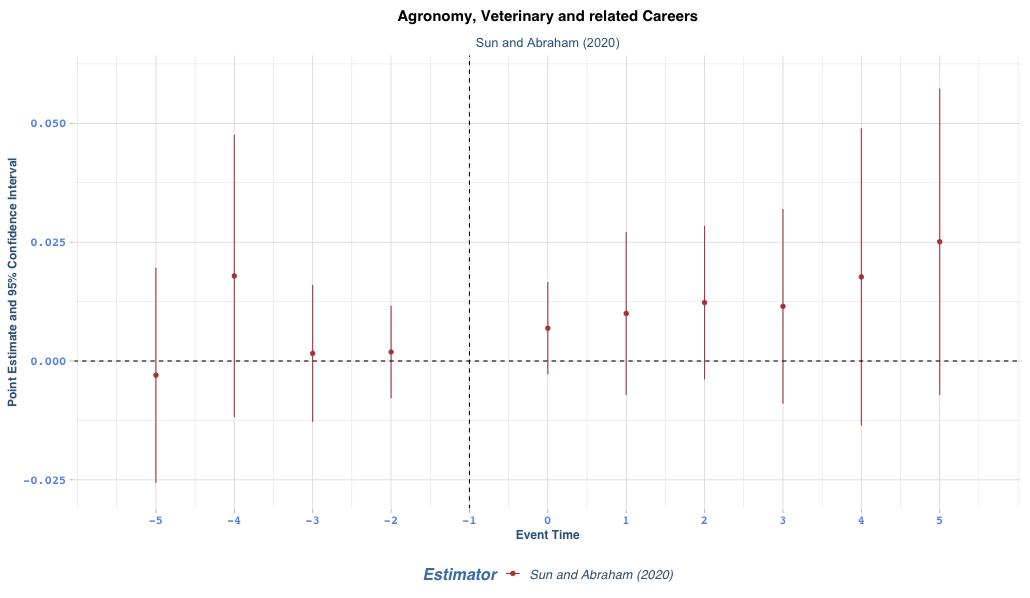
\includegraphics[width=\textwidth]{Graph/Results/stagered_ex_females_AGRONOMY_VETERINARY_RELATED.png}
        \caption{Ex female schools }
        \label{fig:staggered_females_education_sciences1}
    \end{subfigure}
    \hfill
    \begin{subfigure}[b]{0.45\textwidth}
        \centering
        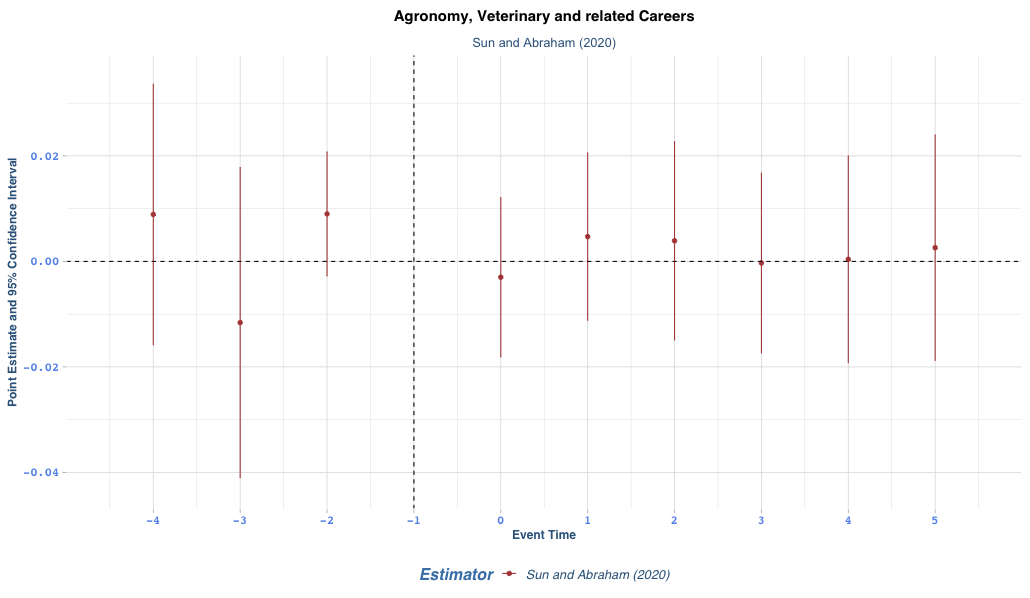
\includegraphics[width=\textwidth]{Graph/Results/stagered_ex_males_AGRONOMY_VETERINARY_RELATED.png}
        \caption{Ex male schools}
        \label{fig:staggered_males_education_sciences2}
    \end{subfigure}
       \caption{ Changes in the Proportion of Students Choosing Education Sciences Majors  in Schools Transitioning from Single-Sex to Coeducational}
    \label{fig:staggered_education_sciences1}
\end{figure}

\begin{figure}[H]
\centering
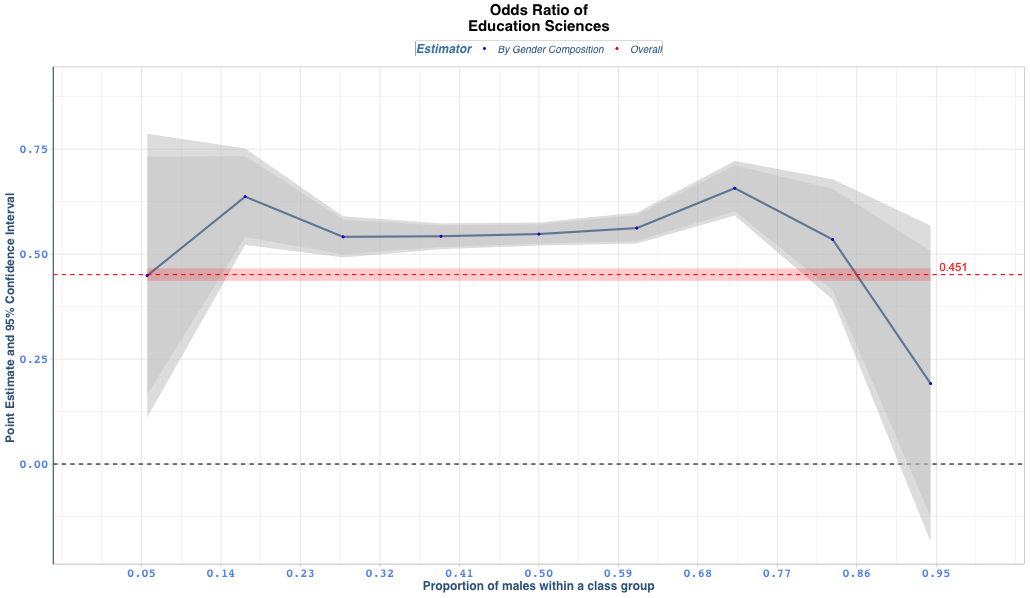
\includegraphics[width=0.8\textwidth]{Graph/Results/fe_panel_student_gender_composition_wome_in_EDUCATION_SCIENCES_bce.png}
\caption{Likelihood of a female student choosing education sciences majors}
\label{fig:education_sciences}
\end{figure}

4. \textbf{Health Sciences Majors (Except Medicine)}: The odds ratio for female students opting for majors in health sciences exhibits variability with changes in the male composition fraction in the classroom. Similar to some other fields, higher proportions of male students are associated with higher odds ratios, suggesting a potential preference among female students for these majors in more gender-diverse environments.

\begin{figure}[H]
    \centering
    \begin{subfigure}[b]{0.45\textwidth}
        \centering
        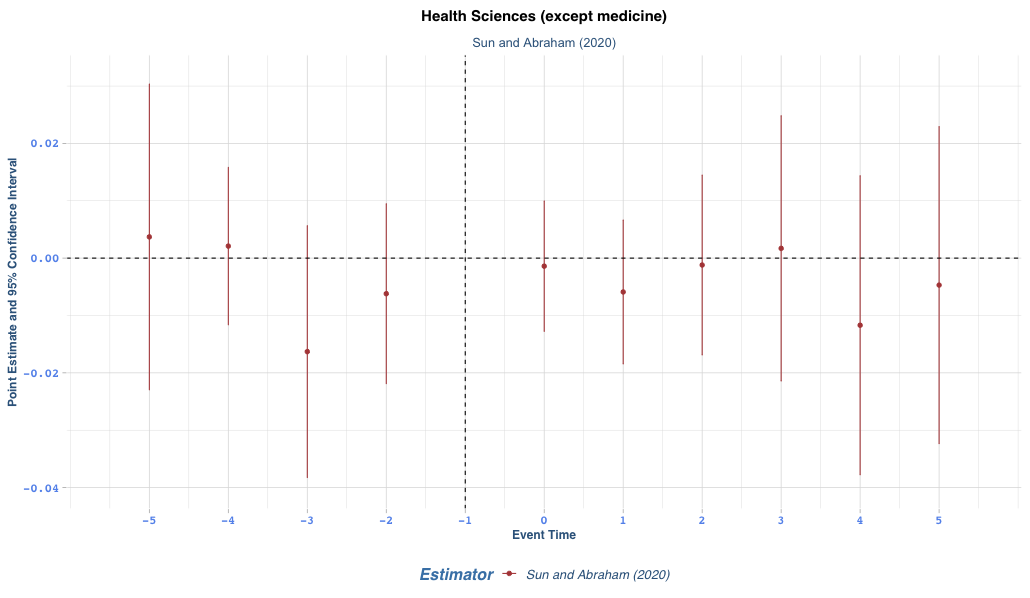
\includegraphics[width=\textwidth]{Graph/Results/stagered_ex_females_HEALTH_SCIENCES.png}
        \caption{Ex female schools }
        \label{fig:staggered_females_health_sciences}
    \end{subfigure}
    \hfill
    \begin{subfigure}[b]{0.45\textwidth}
        \centering
        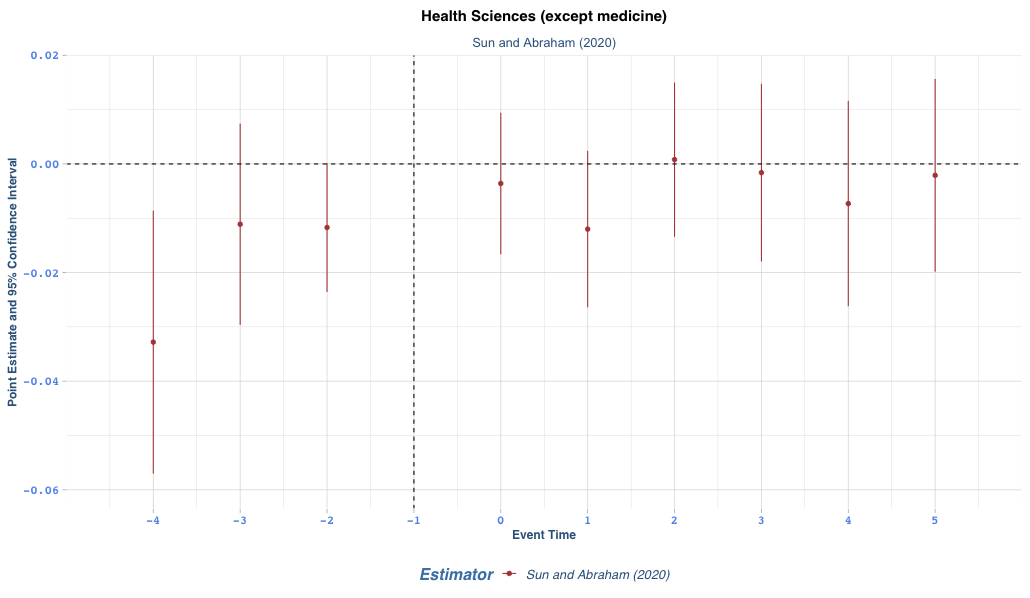
\includegraphics[width=\textwidth]{Graph/Results/stagered_ex_males_HEALTH_SCIENCES.png}
        \caption{Ex male schools}
        \label{fig:staggered_males_health_sciences}
    \end{subfigure}
       \caption{ Changes in the Proportion of Students Choosing Health Science Majors (Except Medicine) in Schools Transitioning from Single-Sex to Coeducational}
    \label{fig:staggered_health_sciences}
\end{figure}

\begin{figure}[H]
\centering
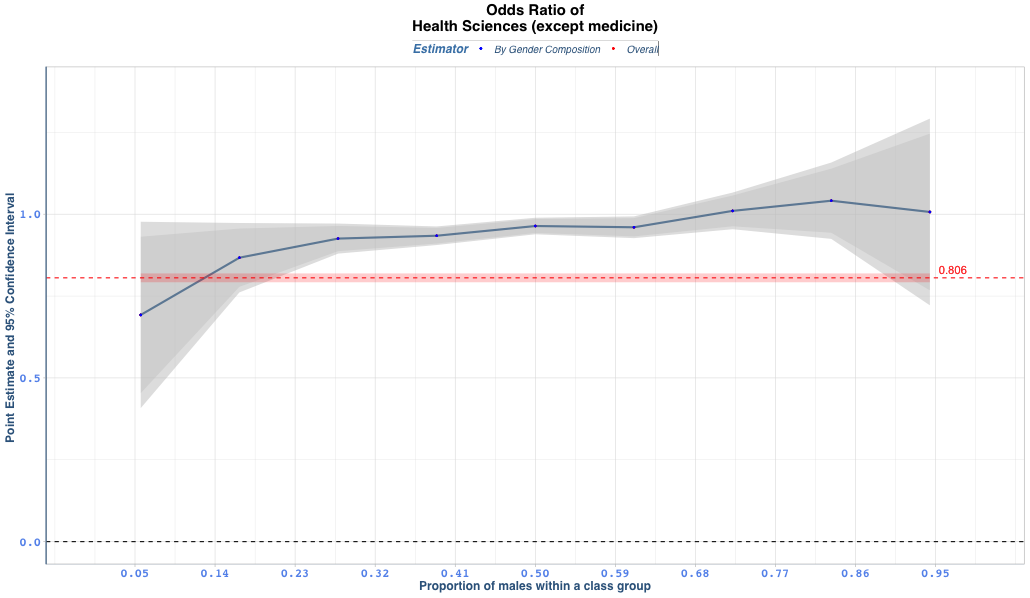
\includegraphics[width=0.8\textwidth]{Graph/Results/fe_panel_student_gender_composition_wome_in_HEALTH_SCIENCES_bce.png}
\caption{Likelihood of a female student choosing health sciences majors}
\label{fig:health_sciences}
\end{figure}




5. \textbf{Medicine Major}: The odds ratio for female students selecting majors in medicine fluctuates with changes in the male composition fraction in the classroom. Higher proportions of male students are associated with lower odds ratios, suggesting potential barriers or deterrents for female students in pursuing medicine majors in more male-dominated environments.

\begin{figure}[H]
    \centering
    \begin{subfigure}[b]{0.45\textwidth}
        \centering
        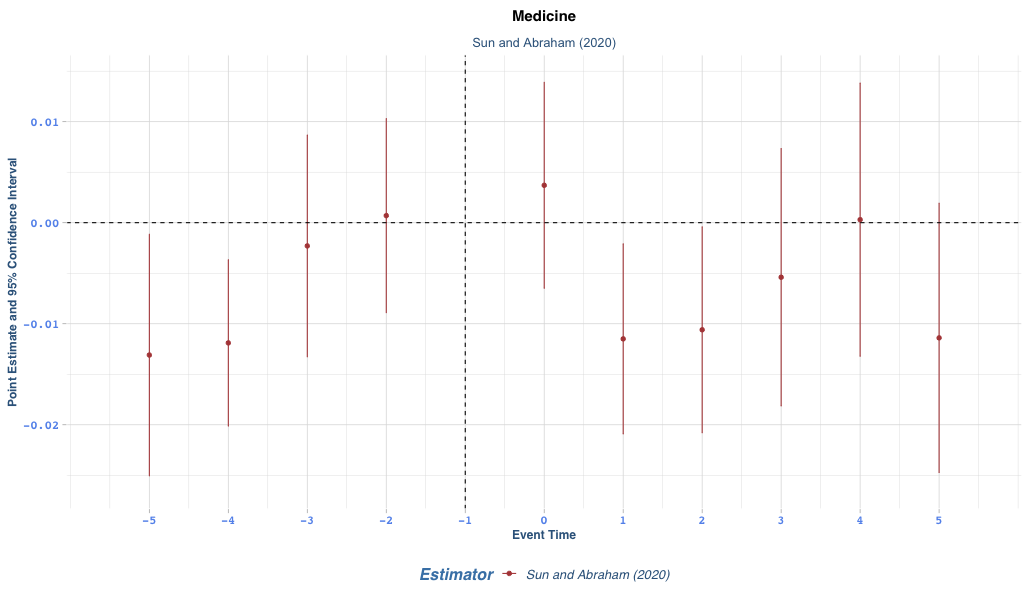
\includegraphics[width=\textwidth]{Graph/Results/stagered_ex_females_MEDICINE.png}
        \caption{Ex female schools }
        \label{fig:staggered_females_medicine}
    \end{subfigure}
    \hfill
    \begin{subfigure}[b]{0.45\textwidth}
        \centering
        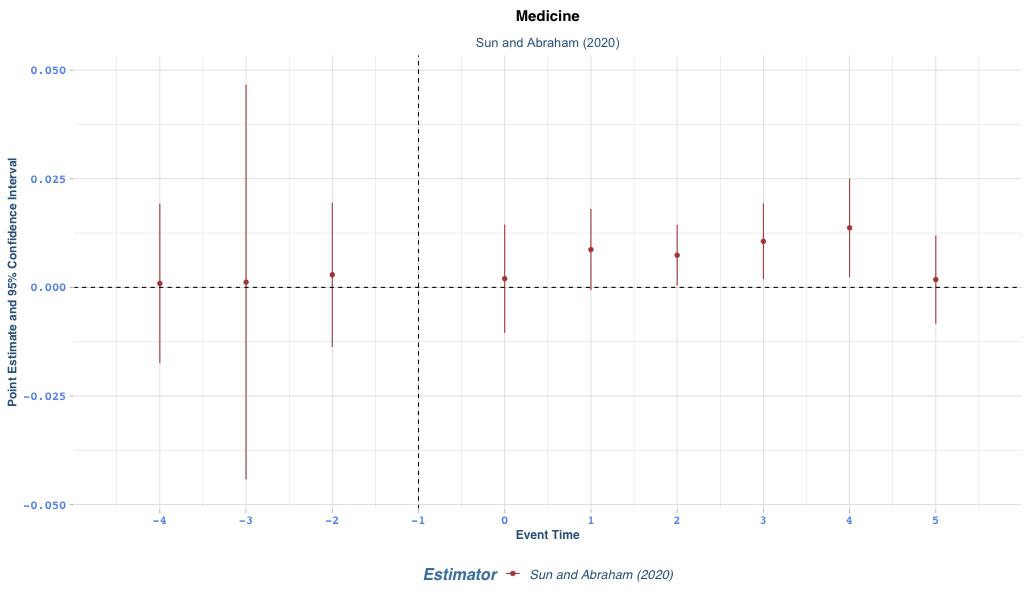
\includegraphics[width=\textwidth]{Graph/Results/stagered_ex_males_MEDICINE.png}
        \caption{Ex male schools}
        \label{fig:staggered_males_medicine}
    \end{subfigure}
       \caption{ Changes in the Proportion of Students Choosing A Major in Medicine from Schools Transitioning from Single-Sex to Coeducational}
    \label{fig:staggered_medicine}
\end{figure}

\begin{figure}[H]
\centering
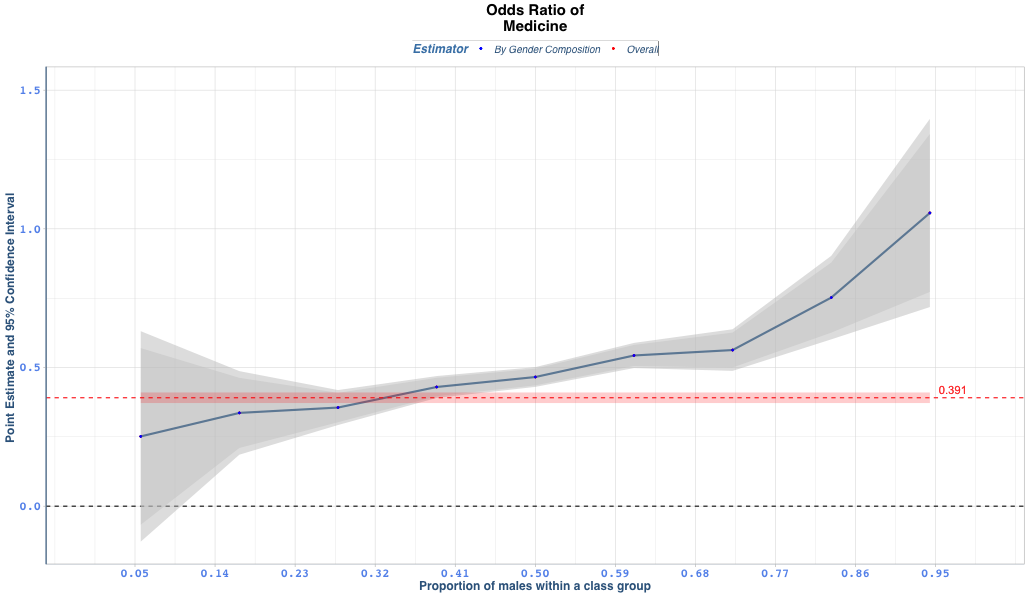
\includegraphics[width=0.8\textwidth]{Graph/Results/fe_panel_student_gender_composition_wome_in_MEDICINE_bce.png}
\caption{Likelihood of a female student choosing medicine majors}
\label{fig:medicine}
\end{figure}

6. \textbf{Law Majors}: The odds ratio for female students opting for majors in law demonstrates variability with changes in the male composition fraction in the classroom. Higher proportions of male students are associated with higher odds ratios, suggesting a potential preference among female students for these majors in more gender-diverse environments.

\begin{figure}[H]
    \centering
    \begin{subfigure}[b]{0.45\textwidth}
        \centering
        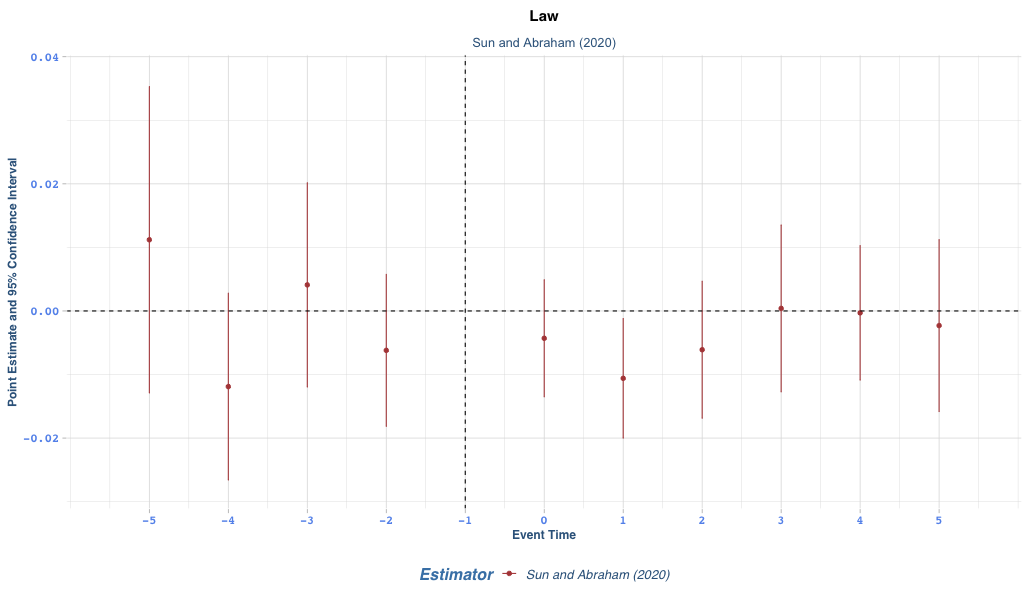
\includegraphics[width=\textwidth]{Graph/Results/stagered_ex_females_LAW.png}
        \caption{Ex female schools }
        \label{fig:staggered_females_education_sciences}
    \end{subfigure}
    \hfill
    \begin{subfigure}[b]{0.45\textwidth}
        \centering
        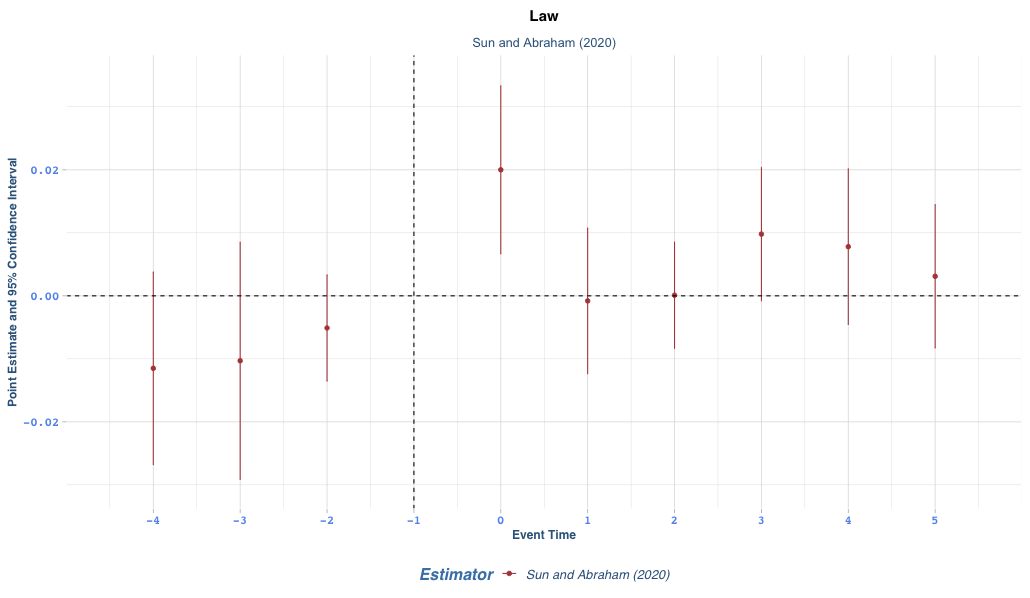
\includegraphics[width=\textwidth]{Graph/Results/stagered_ex_males_LAW.png}
        \caption{Ex male schools}
        \label{fig:staggered_males_education_sciences}
    \end{subfigure}
       \caption{ Changes in the Proportion of Students Choosing  a Major in LAW in Schools Transitioning from Single-Sex to Coeducational}
    \label{fig:staggered_education_sciences}
\end{figure}

\begin{figure}[htbp]
\centering
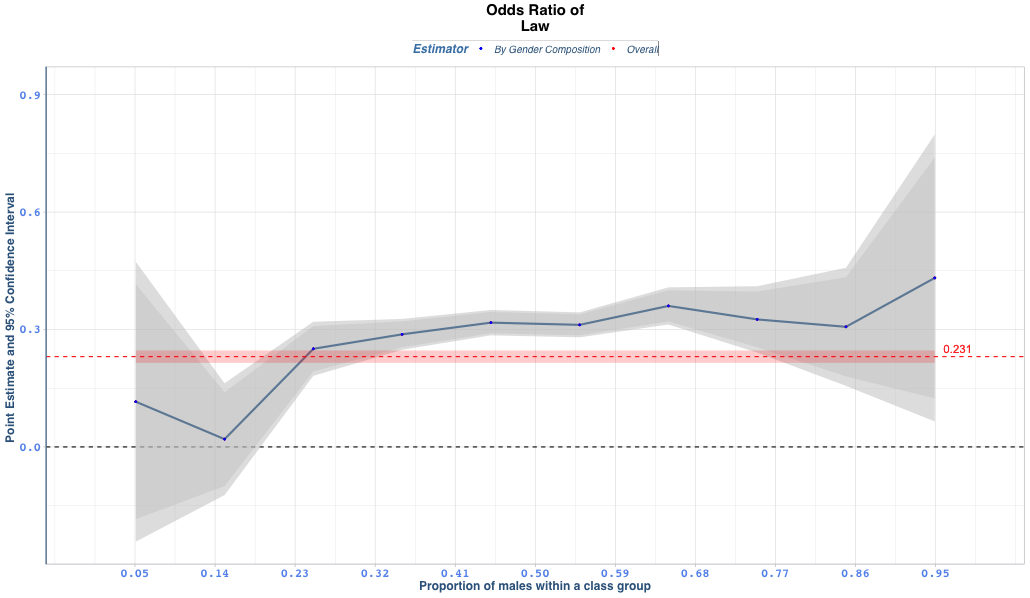
\includegraphics[width=0.8\textwidth]{Graph/Results/fe_panel_student_gender_composition_wome_in_LAW_bce.png}
\caption{Likelihood of a female student choosing law majors}
\label{fig:law}
\end{figure}

\subsubsection{Fields of Study  Less Preferred by Female Students}\label{subsec:less_preferred_female}

This section examines the fields of study  where female students display a lower preference compared to male students.



 


1. \textbf{Engineering/Architecture Related Majors}: The odds ratio for female students opting for majors in engineering and architecture also exhibits variability based on the male composition fraction in the classroom. Interestingly, as the proportion of male students increases, the odds ratio tends to decrease, suggesting a potential deterrent effect on female students' interest in these fields. This trend highlights the importance of considering classroom demographics in understanding gender disparities in engineering and architecture-related majors.

 
\begin{figure}[H]
    \centering
    \begin{subfigure}[b]{0.45\textwidth}
        \centering
        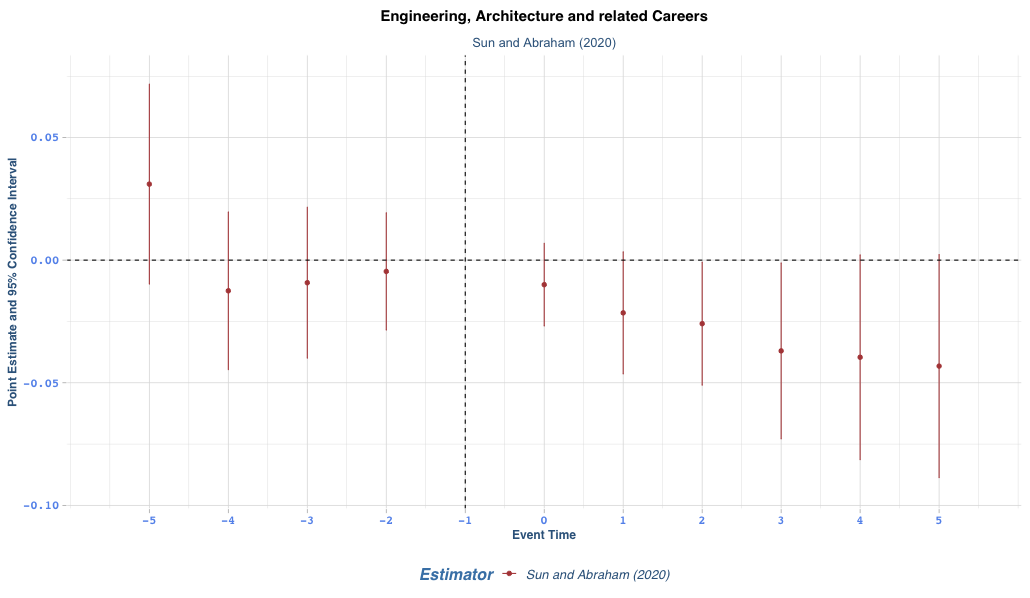
\includegraphics[width=\textwidth]{Graph/Results/stagered_ex_females_ENG_ARCH_RELATED.png}
        \caption{Ex female schools }
        \label{fig:staggered_females_eng}
    \end{subfigure}
    \hfill
    \begin{subfigure}[b]{0.45\textwidth}
        \centering
        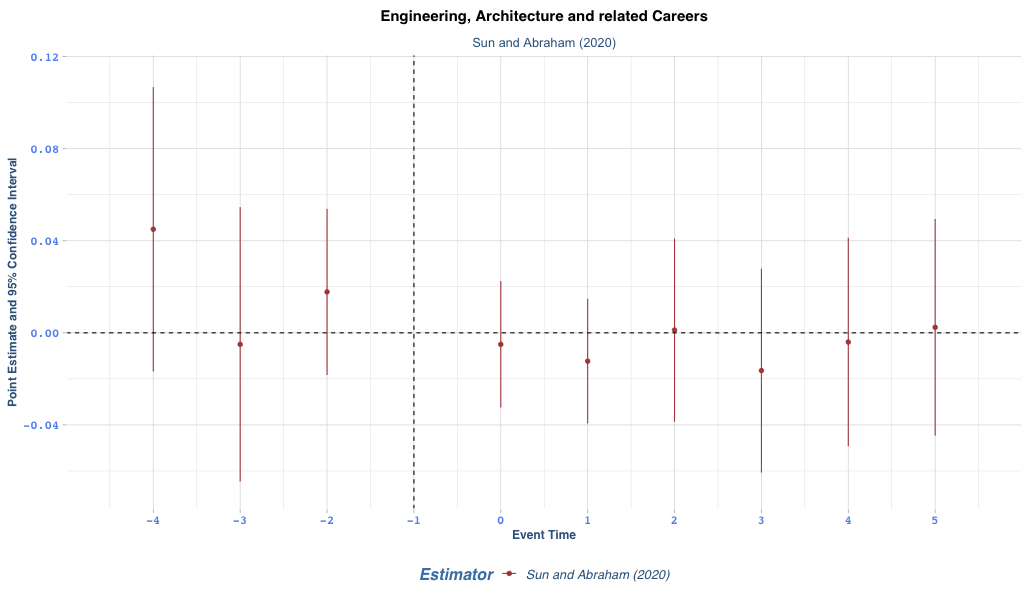
\includegraphics[width=\textwidth]{Graph/Results/stagered_ex_males_ENG_ARCH_RELATED.png}
        \caption{Ex male schools }
        \label{fig:staggered_males_eng}
    \end{subfigure}
\caption{ Changes in the Proportion of Students Choosing Engineering, Architecture and  Related Majors in Schools Transitioning from Single-Sex to Coeducational}
    \label{fig:staggered_eng_arch_related}
\end{figure}

\begin{figure}[H]
\centering
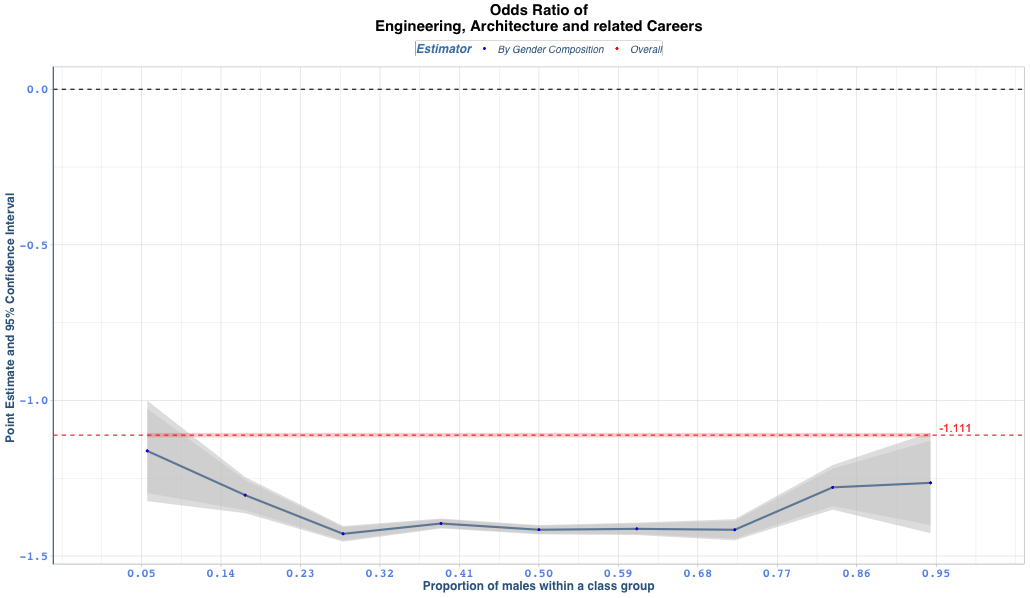
\includegraphics[width=0.8\textwidth]{Graph/Results/fe_panel_student_gender_composition_wome_in_ENG_ARCH_RELATED_bce.png}
\caption{Likelihood of a female student choosing engineering/architecture-related majors}
\label{fig:eng_arch_related}
\end{figure}

% Your analysis goes here

2. \textbf{Mathematics and Natural Sciences Majors}: Similar to other fields, the odds ratio for female students selecting majors in mathematics and natural sciences fluctuates with changes in the male composition fraction. Higher proportions of male students in the classroom are associated with lower odds ratios, suggesting potential barriers or deterrents for female students in pursuing these majors in more male-dominated environments.

\begin{figure}[H]
    \centering
    \begin{subfigure}[b]{0.45\textwidth}
        \centering
        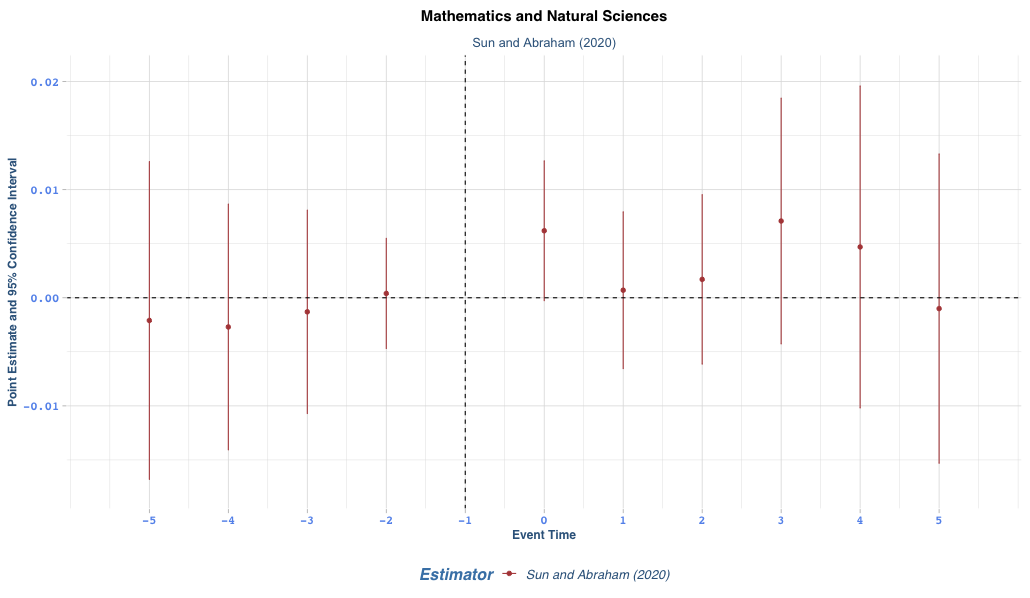
\includegraphics[width=\textwidth]{Graph/Results/stagered_ex_females_MATHEMATICS_NATURAL_SCIENCES.png}
        \caption{Ex female schools }
        \label{fig:staggered_females_math_natural_sciences}
    \end{subfigure}
    \hfill
    \begin{subfigure}[b]{0.45\textwidth}
        \centering
        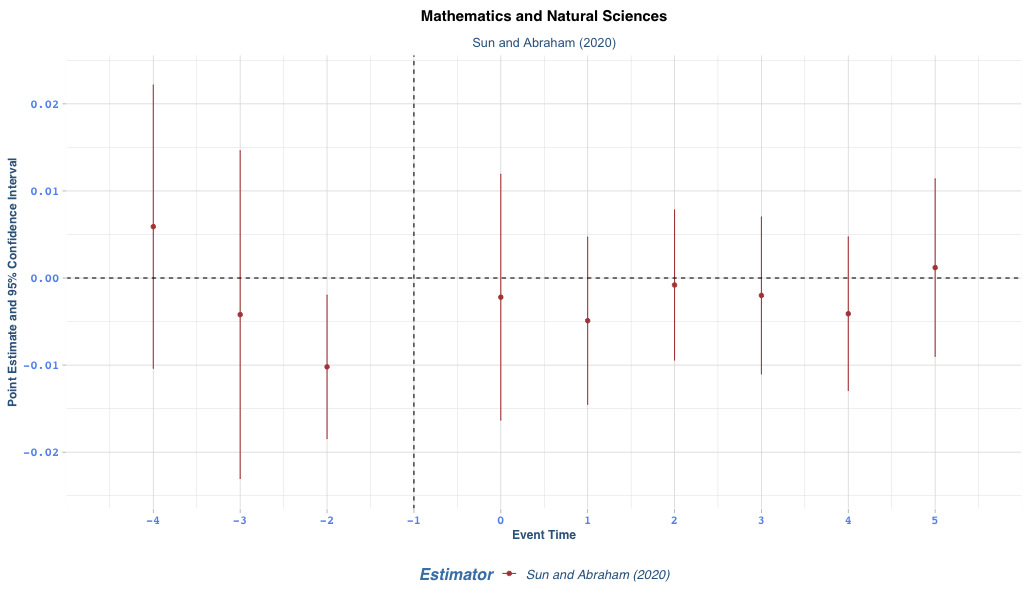
\includegraphics[width=\textwidth]{Graph/Results/stagered_ex_males_MATHEMATICS_NATURAL_SCIENCES.png}
        \caption{Ex male schools }
        \label{fig:staggered_males_math_natural_sciences}
    \end{subfigure}
\caption{ Changes in the Proportion of Students Choosing Mathematics, Natural Sciences and Related Majors   in Schools Transitioning from Single-Sex to Coeducational}
    \label{fig:staggered_math_natural_sciences}
\end{figure}

\begin{figure}[H]
\centering
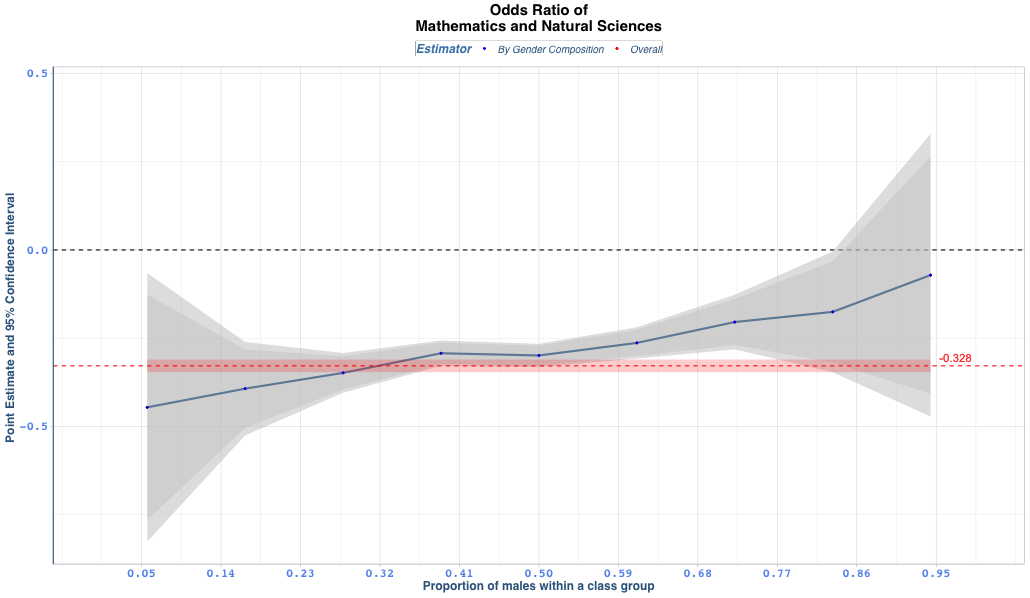
\includegraphics[width=0.8\textwidth]{Graph/Results/fe_panel_student_gender_composition_wome_in_MATHEMATICS_NATURAL_SCIENCES_bce.png}
\caption{Likelihood of a female student choosing mathematics/natural sciences majors}
\label{fig:math_natural_sciences}
\end{figure}



\subsubsection{Fields of Study  with Similar Preferences Between Female and Male Students}\label{subsec:similar_preference}

Here, we explore the fields of study  where both female and male students exhibit similar preferences.
 

 
1. \textbf{Fine Arts Majors}: The odds ratio for female students choosing majors in fine arts demonstrates a less consistent pattern compared to other fields. While there is some fluctuation in the odds ratio with changes in the male composition fraction, the overall trend is less pronounced. Female students seem to exhibit varying preferences for fine arts majors regardless of the gender composition in the classroom.

\begin{figure}[H]
    \centering
    \begin{subfigure}[b]{0.45\textwidth}
        \centering
        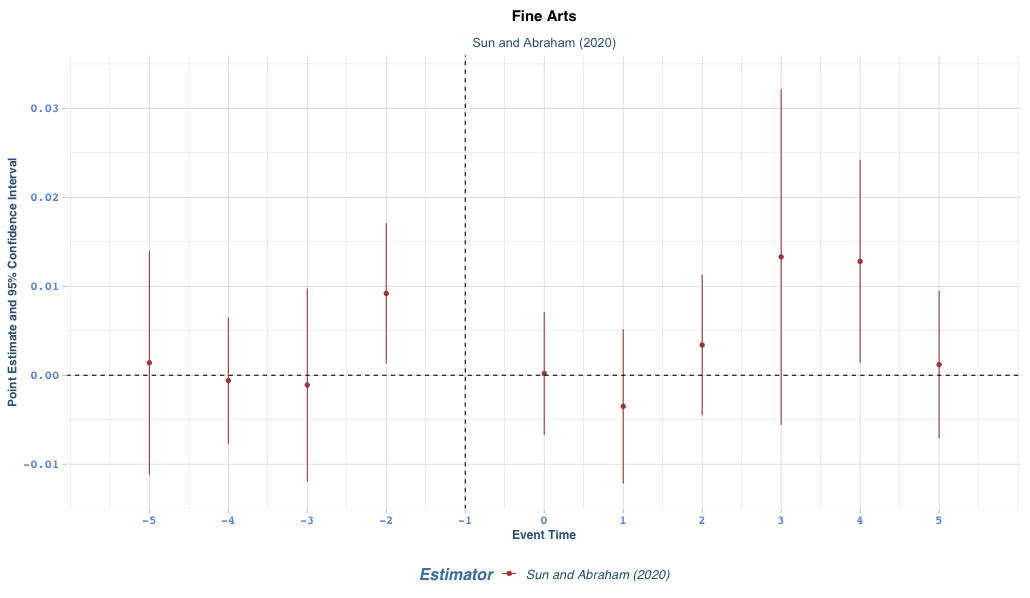
\includegraphics[width=\textwidth]{Graph/Results/stagered_ex_females_FINE_ARTS.png}
        \caption{Ex female schools }
        \label{fig:staggered_females_fine_arts}
    \end{subfigure}
    \hfill
    \begin{subfigure}[b]{0.45\textwidth}
        \centering
        \includegraphics[width=\textwidth]{Graph/Results/stagered_ex_Males_FINE_ARTS.png}
        \caption{Ex male schools }
        \label{fig:staggered_males_fine_arts}
    \end{subfigure}
\caption{ Changes in the Proportion of Students Choosing Fine Arts and Related Majors in Schools Transitioning from Single-Sex to Coeducational}
    \label{fig:staggered_fine_arts}
\end{figure}

\begin{figure}[H]
\centering
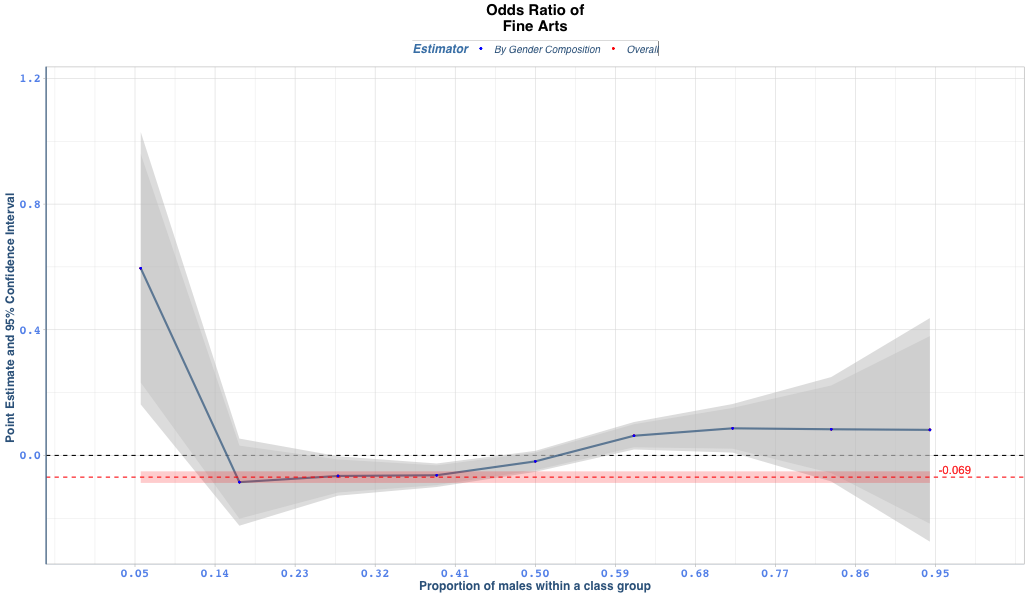
\includegraphics[width=0.8\textwidth]{Graph/Results/fe_panel_student_gender_composition_wome_in_FINE_ARTS_bce.png}
\caption{Likelihood of a female student choosing fine arts majors}
\label{fig:fine_arts}
\end{figure}

2. \textbf{Agronomy/Veterinary Related Majors}: The odds ratio for female students selecting majors in agronomy and veterinary-related fields shows fluctuations with changes in the male composition fraction in the classroom. Higher proportions of male students are associated with lower odds ratios, suggesting potential barriers or deterrents for female students in pursuing these majors in more male-dominated environments.

 
\begin{figure}[H]
    \centering
    \begin{subfigure}[b]{0.45\textwidth}
        \centering
        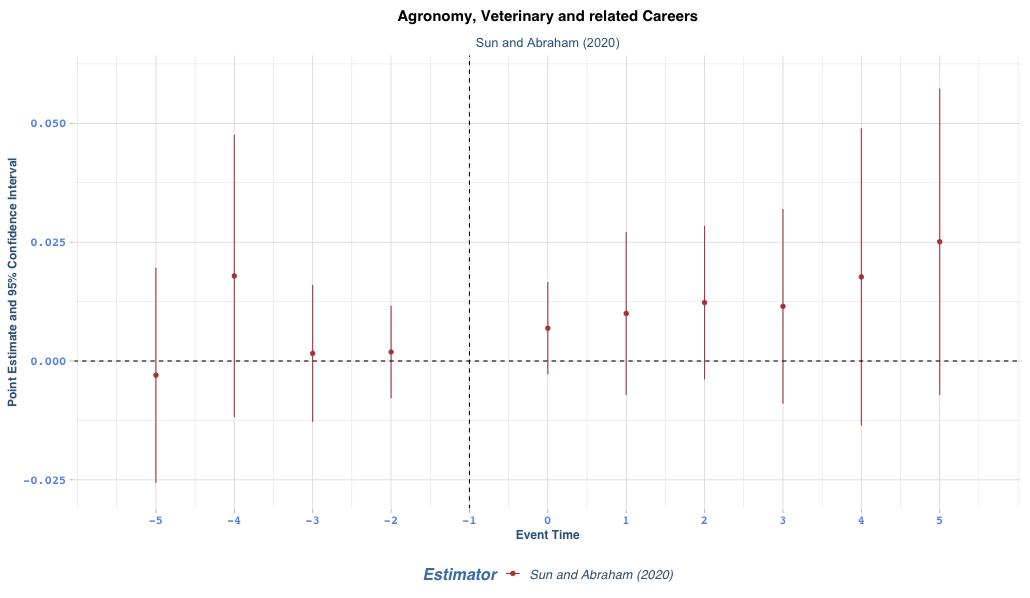
\includegraphics[width=\textwidth]{Graph/Results/stagered_ex_females_AGRONOMY_VETERINARY_RELATED.png}
        \caption{Ex female schools }
        \label{fig:staggered_females_agronomy_veterinary}
    \end{subfigure}
    \hfill
    \begin{subfigure}[b]{0.45\textwidth}
        \centering
        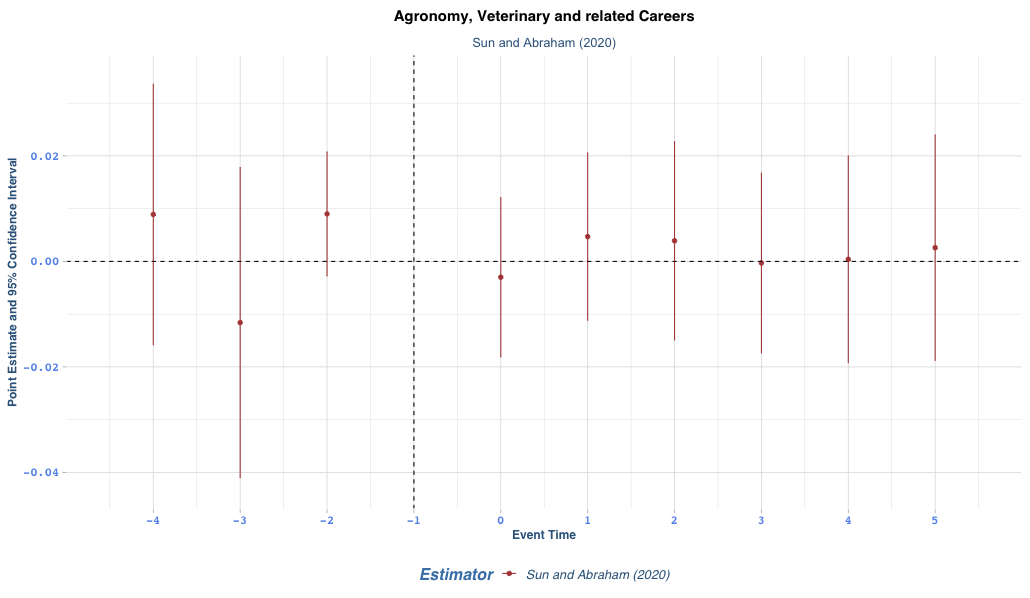
\includegraphics[width=\textwidth]{Graph/Results/stagered_ex_males_AGRONOMY_VETERINARY_RELATED.png}
        \caption{Ex male schools}
        \label{fig:staggered_males_agronomy_veterinary}
    \end{subfigure}
       \caption{ Changes in the Proportion of Students Choosing Agronomy, Veterinary, and Related Majors in Schools Transitioning from Single-Sex to Coeducational}
    \label{fig:staggered_agronomy_veterinary}
\end{figure}


 
\begin{figure}[H]
\centering
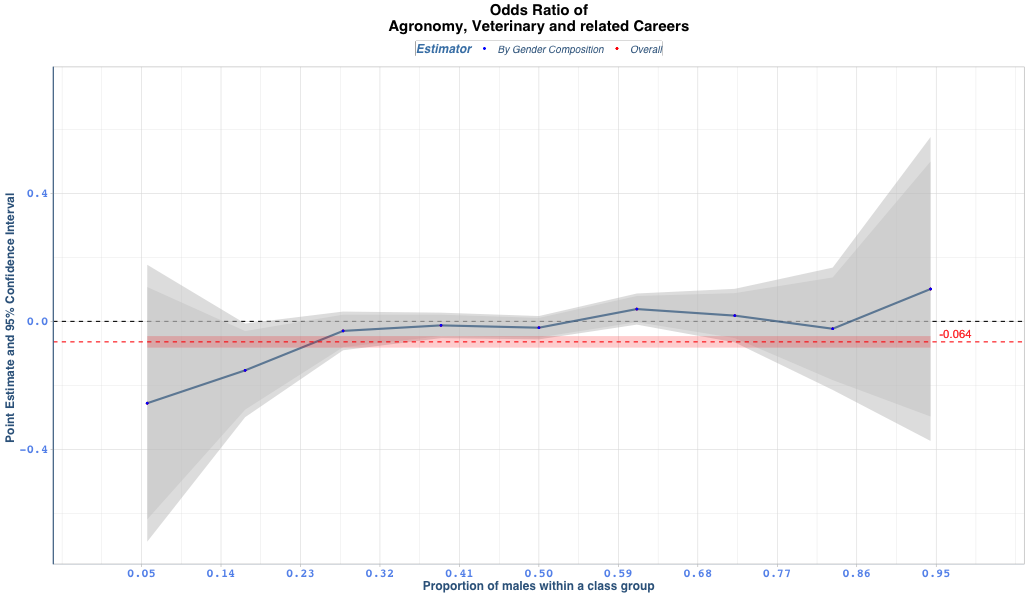
\includegraphics[width=0.8\textwidth]{Graph/Results/fe_panel_student_gender_composition_wome_in_AGRONOMY_VETERINARY_RELATED_bce.png}
\caption{Likelihood of a female student choosing agronomy/veterinary-related majors}
\label{fig:agronomy_veterinary_related}
\end{figure}

% \subsection{-----}
\subsection{Description of University Major Choices by Knowledge Areas} \label{app:path}

This section provides an overview of university major choices categorized into distinct knowledge areas. The aggregated classification is structured as follows:
    \begin{itemize}
        \item 1. Economics, Business \& related Careers ( e.g., Economics, Business Administration, Finance, Accounting, Marketing, Management, Entrepreneurship, International Business, Human Resources)
        \item 2. Engineering, Architecture \ and related Careers (e.g., Civil Engineering, Mechanical Engineering, Electrical Engineering, Architecture, Computer Science, Information Technology, Software Engineering, Industrial Design, Environmental Engineering, Biomedical Engineering)
        \item 3. Fine Arts (Visual Arts, Performing Arts (e.g., Theater, Dance, Music), Graphic Design, Interior Design, Animation)
        \item 4. Mathematics and Natural Sciences (e.g., Mathematics, Physics, Chemistry, Biology, Environmental Science, Geology, Astronomy, Statistics)
        \item 5. Social Sciences and Humanities (e.g.,  Sociology, Anthropology, History, Political Science, Geography, Literature, Philosophy, Religious Studies, Linguistics, Communication Studies)
        \item 6. Agronomy, Veterinary \ and related Careers (e.g., Agronomy, Animal Science, Veterinary Medicine, Zoology, Horticulture, Fisheries and Aquaculture)
        \item 7. Education Sciences (e.g.,  Early Childhood Education, Special Education, Educational Psychology, Education in Mathematics, Education in Sciences ) 
        \item 8. Health Sciences (e.g.,  Nursing, Dentistry, Pharmacy, Physical Therapy, Occupational Therapy, Public Health, Nutrition, Biomedical Sciences, Health Administration,)
        \item 9. No Studies (The student does not continue with professional studies)
    \end{itemize}
\begin{table}[!htbp]
  \centering
  \caption{Correlation between Gender Composition in a Class and Likelihood of Choosing a Career}
  \label{tab:tab1}
  \begin{tabular}{lcccccccccc}
    \toprule
    & \multicolumn{9}{c}{\textit{Dependent variable: Likelihood of Choosing Career}} \\
    \cmidrule(lr){2-10} 
    & (1) & (2) & (3) & (4) & (5) & (6) & (7) & (8) & (9) \\
    \midrule
    Proportion of Males & -0.931*** & 0.982*** & -0.200*** & -0.436*** & -0.996*** & -0.011 & -0.707*** & -1.119*** & 0.445*** \\
    & (0.010) & (0.009) & (0.026) & (0.026) & (0.012) & (0.026) & (0.021) & (0.015) & (0.006) \\
    \addlinespace
    Constant & -1.828*** & -2.535*** & -4.285*** & -4.176*** & -2.407*** & -4.335*** & -3.658*** & -2.732*** & 0.385*** \\
    & (0.005) & (0.005) & (0.013) & (0.012) & (0.006) & (0.012) & (0.010) & (0.007) & (0.003) \\
    \midrule
    Observations & \multicolumn{1}{c}{4,486,601} & \multicolumn{1}{c}{4,486,601} & \multicolumn{1}{c}{4,486,601} & \multicolumn{1}{c}{4,486,601} & \multicolumn{1}{c}{4,486,601} & \multicolumn{1}{c}{4,486,601} & \multicolumn{1}{c}{4,486,601} & \multicolumn{1}{c}{4,486,601} & \multicolumn{1}{c}{4,486,601} \\
    Log Likelihood & \multicolumn{1}{c}{-1,412,835.0} & \multicolumn{1}{c}{-1,562,897.0} & \multicolumn{1}{c}{-299,879.8} & \multicolumn{1}{c}{-300,436.7} & \multicolumn{1}{c}{-947,917.1} & \multicolumn{1}{c}{-308,616.4} & \multicolumn{1}{c}{-411,800.1} & \multicolumn{1}{c}{-723,508.2} & \multicolumn{1}{c}{-2,921,328.0} \\
    AIC & \multicolumn{1}{c}{2,825,674.0} & \multicolumn{1}{c}{3,125,798.0} & \multicolumn{1}{c}{599,763.7} & \multicolumn{1}{c}{600,877.4} & \multicolumn{1}{c}{1,895,838.0} & \multicolumn{1}{c}{617,236.9} & \multicolumn{1}{c}{823,604.2} & \multicolumn{1}{c}{1,447,020.0} & \multicolumn{1}{c}{5,842,660.0} \\
    \bottomrule
  \end{tabular}
\begin{threeparttable}
  \begin{tablenotes}
  \small
    \item Note: $^{*}$p$<$0.1; $^{**}$p$<$0.05; $***$p$<$0.01 
  \end{tablenotes}
  \end{threeparttable}
\end{table}

\newpage
 \subsection{Optimal bandwidth estimation based on Binary cross-entropy }
 \label{bce}

In order to analyze the probability that a secondary school student chooses an field of study  $P$ to pursue post-secondary studies. We analyze the probability according to different gender compositions in the classrooms. Therefore we assume that exists a fixed value that allow to subset by $\exists X_{\text{optimal}}$  The formal representation using mathematical notation for the partitioning of the range into fixed intervals:
Let $X_i$ be a subset that belongs to the gender composition with values between [0,1], we can say that, $X_1$ is a subset that goes from $\min(X)$ to $\min(X)$+$X_i$, consequently $X_2$ is a subset which goes from $X_1$ to $X_1$+$X_i$, and sequentially until $X_n$ goes from $X_{n_{-1}}$ to $\max(X)$.



Let \( X_{\text{optimal}} \) be a fixed interval representing the space between each subset.

The subsets \( X_i \) can be defined as:

 
\begin{align*}
X_1 &= [0, X_{\text{optimal}}) \\
X_2 &= [X_{\text{optimal}}, 2X_{\text{optimal}}) \\
X_3 &= [2X_{\text{optimal}}, 3X_{\text{optimal}}) \\
& \ldots \\
X_n &= [(n-1)X_{\text{optimal}}, nX_{\text{optimal}})
\end{align*}
  

% Where:
% - \( X_1 \) starts from 0 and extends up to \( X_{\text{optimal}} \).
% - \( X_2 \) starts from \( X_{\text{optimal}} \) and extends up to \( 2X_{\text{optimal}} \).
% - \( X_3 \) starts from \( 2X_{\text{optimal}} \) and extends up to \( 3X_{\text{optimal}} \).
% - And so on, until \( X_n \) starts from \( (n-1)X_{\text{optimal}} \) and extends up to \( nX_{\text{optimal}} \).

These representations \( X_i \) cover the entire range in fixed intervals of \( X_{\text{optimal}} \) and define distinct subsets, each representing an interval of size \( X_{\text{optimal}} \) within the overall range. 

To estimate \( X_{\text{optimal}} \) we modify the methodology proposed in \citet{IMBENS2012}, In it, the key step is to replace the mean squared error (MSE) criterion with a BCE-based criterion.
%%%%%%%%%%%%%%%%%%%%


The key outcome we are trying to predict is a binary variable indicating whether a student chooses a particular area of study (e.g. science, humanities etc) or not. Let's call this $Y_i \in {0, 1}$.

$Y_i = 1$ means student $i$ chose that area of study
$Y_i = 0$ means they did not choose that area.
Our regression discontinuity model is estimating the probability $p_i = P(Y_i = 1 | X_i)$  that the student chooses that area, conditioned on the gender composition in classrooms $X_i$.

Let's call this estimated probability $m(X_i)$, which depends on the bandwidth $h$.

The BCE loss for a single data point measures how well our model is estimating this probability. It is:
\begin{equation}
    \text{BCE}_i = \begin{cases}
-\log(m(X_i)), & \text{if } Y_i = 1\\
-\log(1 - m(X_i)), & \text{if } Y_i = 0
\end{cases}
\end{equation}
 

Penalizes underestimating probability if actual outcome is 1
Penalizes overestimating probability if actual outcome is 0
We then define the overall expected BCE loss over the distribution of $(X_i, Y_i)$ as:

$$\text{BCE}(h) = E[-Y_i \log(m(X_i)) - (1-Y_i)\log(1-m(X_i))]$$

Minimizing this BCE(h) gives the optimal bandwidth for our RD model.
 

\textbf{ 1. Define the BCE Loss Function:}

The key outcome we are trying to predict is a binary variable indicating whether a student chooses a particular area of study (e.g. science, humanities etc) or not. Let's call this $Y_i \in {0, 1}$.

$Y_i = 1$ means student $i$ chose that area of study
$Y_i = 0$ means they did not choose that area.
Our regression discontinuity model is estimating the probability $p_i = P(Y_i = 1 | X_i)$  that the student chooses that area, conditioned on the gender composition in classrooms $X_i$.

Let's call this estimated probability $m(X_i)$, which depends on the bandwidth $h$.

The BCE loss for a single data point measures how well our model is estimating this probability. It is:

\begin{equation}
    \text{BCE}_i = \begin{cases}
-\log(m(X_i)), & \text{if } Y_i = 1\\
-\log(1 - m(X_i)), & \text{if } Y_i = 0
\end{cases}
\end{equation}

 

Penalizes underestimating probability if actual outcome is 1
Penalizes overestimating probability if actual outcome is 0
We then define the overall expected BCE loss over the distribution of $(X_i, Y_i)$ as:

$$\text{BCE}(h) = E[-Y_i \log(m(X_i)) - (1-Y_i)\log(1-m(X_i))]$$

Minimizing this BCE(h) gives the optimal bandwidth for our RD model.



\textbf{ 2. Approximate BCE:}
We have defined the BCE loss as:

$$\text{BCE}(h) = E[-Y_i \log(m(X_i)) - (1-Y_i)\log(1-m(X_i))]$$

However, we cannot directly optimize this BCE(h) to find the best bandwidth h. The expectation over (Xi, Yi) pairs and dependence on the regression function m(Xi) is too complicated.

So we take a Taylor expansion of BCE(h) around the point h=0. This allows us to approximate BCE(h) for small values of h (which is the relevant range for bandwidth selection).

Specifically:

\begin{align*}
\text{BCE}(h) &= \text{BCE}(0) + \text{BCE}'(0)h + \frac{1}{2}\text{BCE}''(0)h^2 + \frac{1}{6}\text{BCE}'''(0)h^3 + O(h^4)\\
&\approx \text{BCE}(0) + \text{BCE}'(0)h + \frac{1}{2}\text{BCE}''(0)h^2
\end{align*}

We assume higher order terms are negligible. After substituting the derivatives, this second order approximation takes the form:

$$\text{AMSE}\text{BCE}(h) = C_1h^4(m''(c)-m''-(c))^2 + \frac{C_2}{Nh}$$

Where:

$C_1, C_2$ depend on moments of Y distribution and kernel
$m''$ and $m''_-$ are second derivatives of the regression function
This $\text{AMSE}_\text{BCE}(h)$ can now be optimized tractably to find the best bandwidth h. It maintains the key structure and tradeoff between variance and bias squared terms.

\textbf{Minimize Approximate BCE:}
In the previous step, we derived the approximate BCE loss function:

$$\text{AMSE}\text{BCE}(h) = C_1h^4(m''(c)-m''-(c))^2 + \frac{C_2}{Nh}$$

This approximate loss maintains the core structure from the MSE case - having a bias squared term that increases with $h$ and a variance term that decreases with $h$.

Our goal now is to find the value of $h$ that minimizes this loss, balancing the bias-variance tradeoff. We can find this by taking the derivative with respect to $h$ and setting it equal to zero:

$$\frac{d}{dh}\text{AMSE}\text{BCE}(h) = 4C_1h^3(m''(c)-m''-(c))^2 - \frac{C_2}{Nh^2}$$

Setting this equal to zero gives us the optimal bandwidth that minimizes the approximate BCE:

$$h_\text{opt, BCE} = \left(\frac{C_2}{4C_1}\right)^{\frac{1}{5}} N^{-\frac{1}{5}}$$

We get a very similar expression as in the MSE case, with the leading constant now depending on the BCE-based constants $C_1$ and $C_2$.

This $h_\text{opt, BCE}$ minimizes the approximate expected BCE loss over the distribution of data. Using this bandwidth will give us the regression discontinuity model that best trades off bias vs variance in terms of BCE.

\textbf{Estimate the Bandwidth}

We derived the formula for the optimal bandwidth that minimizes the approximate BCE criterion:

$$h_\text{opt, BCE} = \left(\frac{C_2}{4C_1}\right)^{\frac{1}{5}} N^{-\frac{1}{5}}$$

The issue is this still relies on unknown population quantities - namely the constants $C_1, C_2$ and the second derivatives of the regression function $m''(c)$ and $m_-''(c)$.

So the final step is to estimate these unknowns from the data, in order to obtain a data-driven bandwidth estimate. There are a few options for doing this estimation:

Use pilot estimates: Obtain initial/crude estimates of $C_1, C_2, m'', m_-''$ using some pilot bandwidth $h_\text{pilot}$. These don't need to be very precise.
Moment approximations: Approximate moments of Y distribution and kernel to get estimates of $C_1, C_2$ without directly estimating them.
Iterative/cross-validation: Obtain estimates of the derivatives $m'',m''_-$ using some initial h. Then solve for ĥ opt. Iterate with updated derivative estimates.
Either way, once we plug in these estimates, we get a feasible bandwidth formula:

$$\hat{h}_\text{opt, BCE} = \left(\frac{\hat{C}_2}{4\hat{C}_1}\right)^{\frac{1}{5}} N^{-\frac{1}{5}}$$

This estimated $\hat{h}_\text{opt, BCE}$ consistently estimates the optimal bandwidth and maintains the same asymptotic properties as if the true unknowns were used.
%%%%%%%%%%%%%%%%%%%%%%%%%%%%%%%%%%%%%%%
\subsection{Optimal Distance for Different Major Categories}

In this section, we present the graphs illustrating the optimal distance for different major categories based on the Bayesian Cross Entropy (BCE) metric. Each graph corresponds to a specific academic major category.

Here are the texts for each graph, explaining the optimal distance and its significance:

\textbf{1. Agronomy and Veterinary Related Majors}:
   As depicted in Figure \ref{fig:optimal_distance_agronomy_vet}, the optimal distance that minimizes the entropy in schooling decisions regarding the selection of Agronomy and Veterinary Related Majors is 0.1109.

\begin{figure}[H]
    \centering
    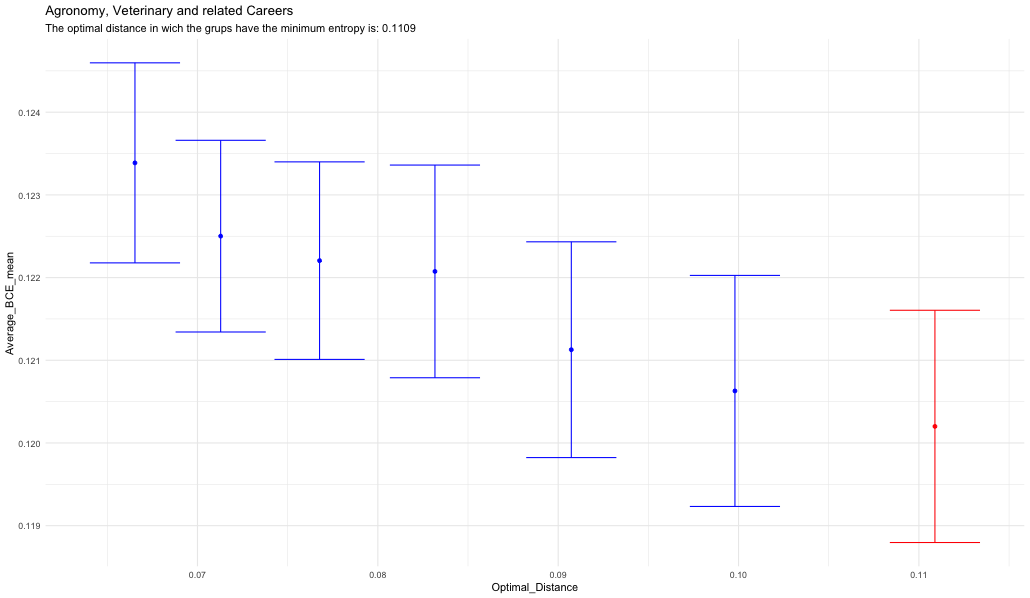
\includegraphics[width=0.8\textwidth]{Graph/Results/optimal_distance_bs30_AGRONOMY_VETERINARY_RELATED.png}
    \caption{Optimal Distance for Agronomy and Veterinary Related Majors}
    \label{fig:optimal_distance_agronomy_vet}
\end{figure}

\textbf{2. Economics and Business Related Majors}:
   Figure \ref{fig:optimal_distance_econ_bus} illustrates that the optimal distance for minimizing entropy in schooling decisions related to Economics and Business majors is 0.0832.

\begin{figure}[H]
    \centering
    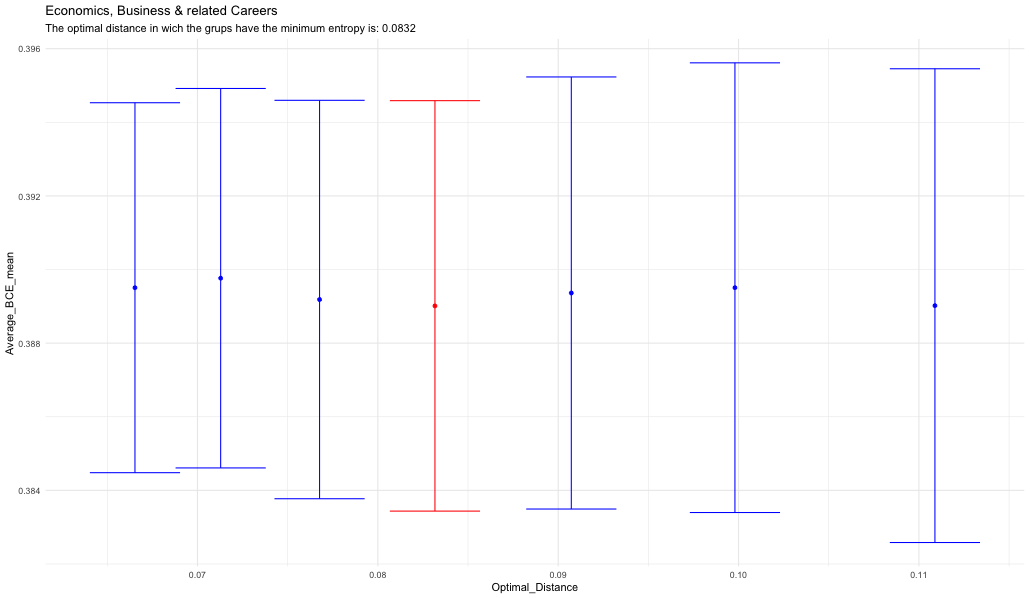
\includegraphics[width=0.8\textwidth]{Graph/Results/optimal_distance_bs30_ECONOMICS_BUSINESS_RELATED.png}
    \caption{Optimal Distance for Economics and Business Related Majors}
    \label{fig:optimal_distance_econ_bus}
\end{figure}

\textbf{ 3. Education Sciences Majors}:
   Examining Figure \ref{fig:optimal_distance_edu_sci}, we find that the optimal distance for Education Sciences majors, which minimizes entropy in schooling decisions, is 0.1109.

\begin{figure}[H]
    \centering
    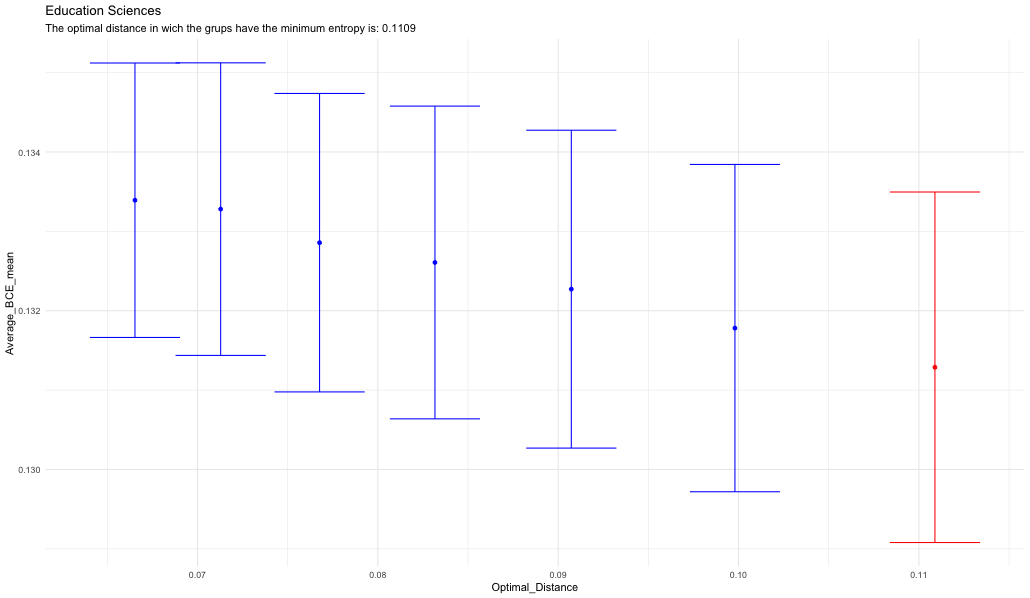
\includegraphics[width=0.8\textwidth]{Graph/Results/optimal_distance_bs30_EDUCATION_SCIENCES.png}
    \caption{Optimal Distance for Education Sciences Majors}
    \label{fig:optimal_distance_edu_sci}
\end{figure}

\textbf{ 4. Engineering and Architecture Related Majors}:
   Figure \ref{fig:optimal_distance_eng_arch} presents the optimal distance of 0.1109 for minimizing entropy in schooling decisions concerning Engineering and Architecture Related Majors.

\begin{figure}[H]
    \centering
    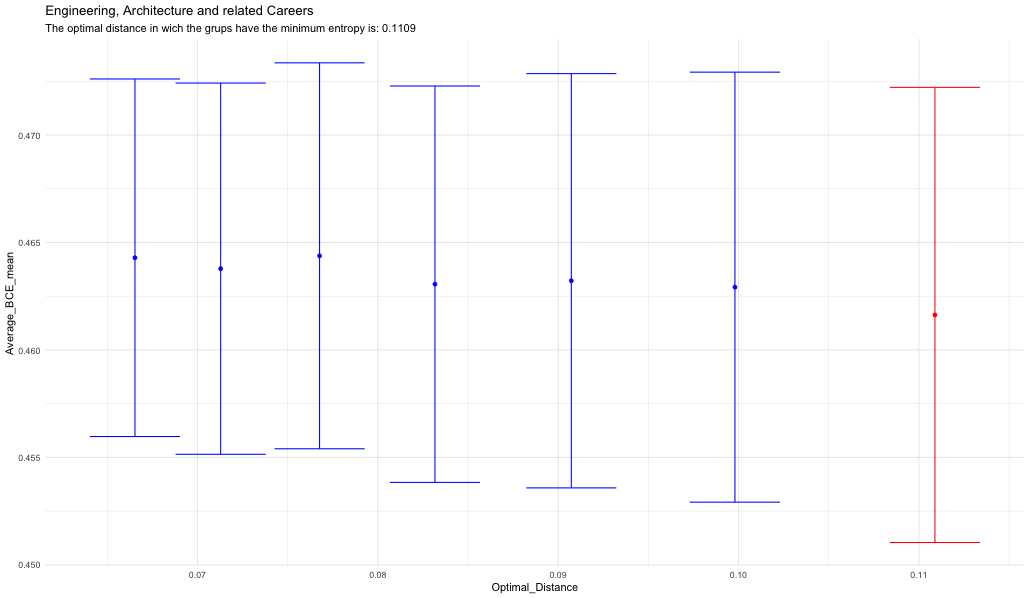
\includegraphics[width=0.8\textwidth]{Graph/Results/optimal_distance_bs30_ENG_ARCH_RELATED.png}
    \caption{Optimal Distance for Engineering and Architecture Related Majors}
    \label{fig:optimal_distance_eng_arch}
\end{figure}

\textbf{5. Fine Arts Majors}:
   In Figure \ref{fig:optimal_distance_fine_arts}, we observe that the optimal distance for minimizing entropy in schooling decisions pertaining to Fine Arts majors is 0.1109.

\begin{figure}[htbp]
    \centering
    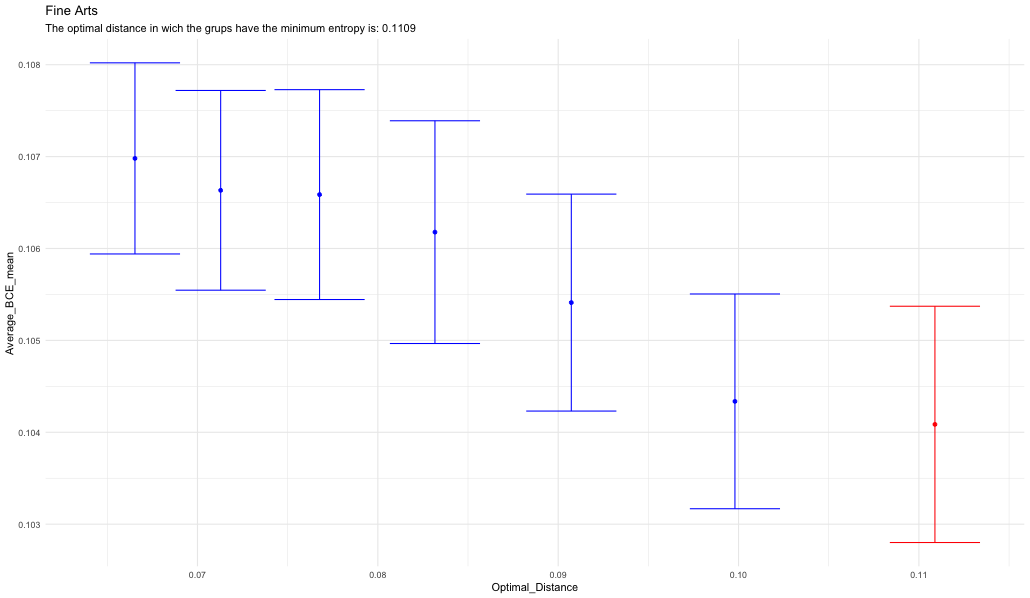
\includegraphics[width=0.8\textwidth]{Graph/Results/optimal_distance_bs30_FINE_ARTS.png}
    \caption{Optimal Distance for Fine Arts Majors}
    \label{fig:optimal_distance_fine_arts}
\end{figure}

\textbf{ 6. Health Sciences Majors}:
   The optimal distance of 0.0832, as shown in Figure \ref{fig:optimal_distance_health_sci}, minimizes entropy in schooling decisions regarding Health Sciences majors.

\begin{figure}[H]
    \centering
    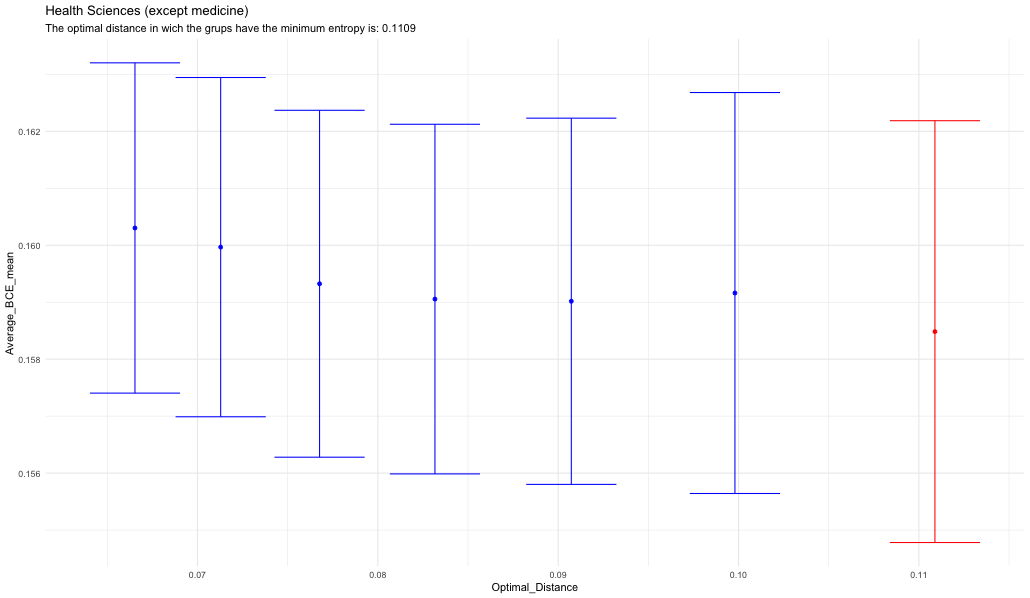
\includegraphics[width=0.8\textwidth]{Graph/Results/optimal_distance_bs30_HEALTH_SCIENCES.png}
    \caption{Optimal Distance for Health Sciences Majors}
    \label{fig:optimal_distance_health_sci}
\end{figure}

\textbf{7. Law Majors}:
   Figure \ref{fig:optimal_distance_law} illustrates that the optimal distance for minimizing entropy in schooling decisions regarding Law majors is 0.0998.

\begin{figure}[H]
    \centering
    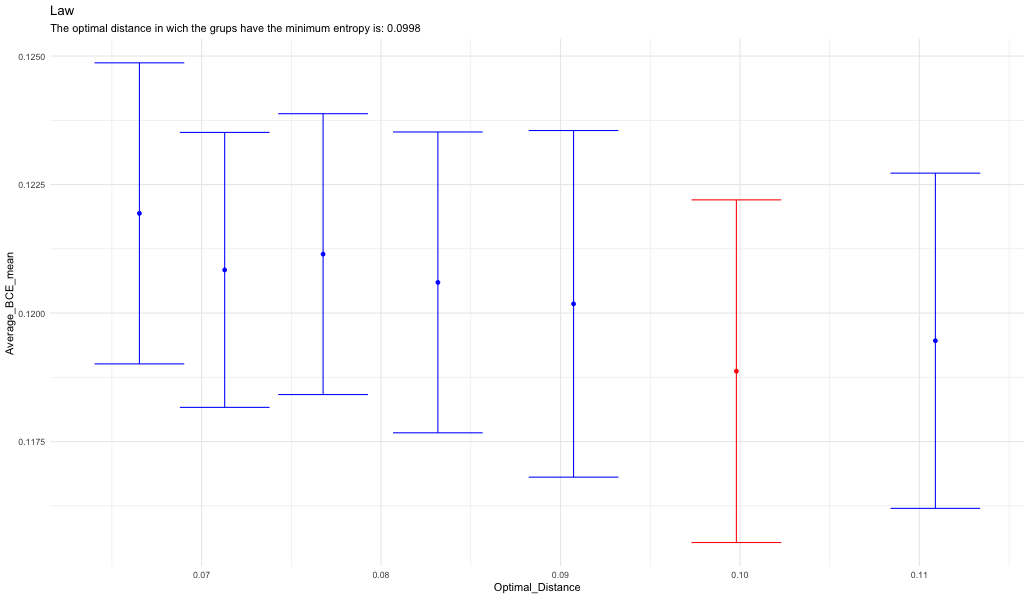
\includegraphics[width=0.8\textwidth]{Graph/Results/optimal_distance_bs30_LAW.png}
    \caption{Optimal Distance for Law Majors}
    \label{fig:optimal_distance_law}
\end{figure}

\textbf{8. Mathematics and Natural Sciences Majors}:
   Examining Figure \ref{fig:optimal_distance_math_natural_sci}, we find that the optimal distance for Mathematics and Natural Sciences majors, which minimizes entropy in schooling decisions, is 0.1109.

\begin{figure}[H]
    \centering
    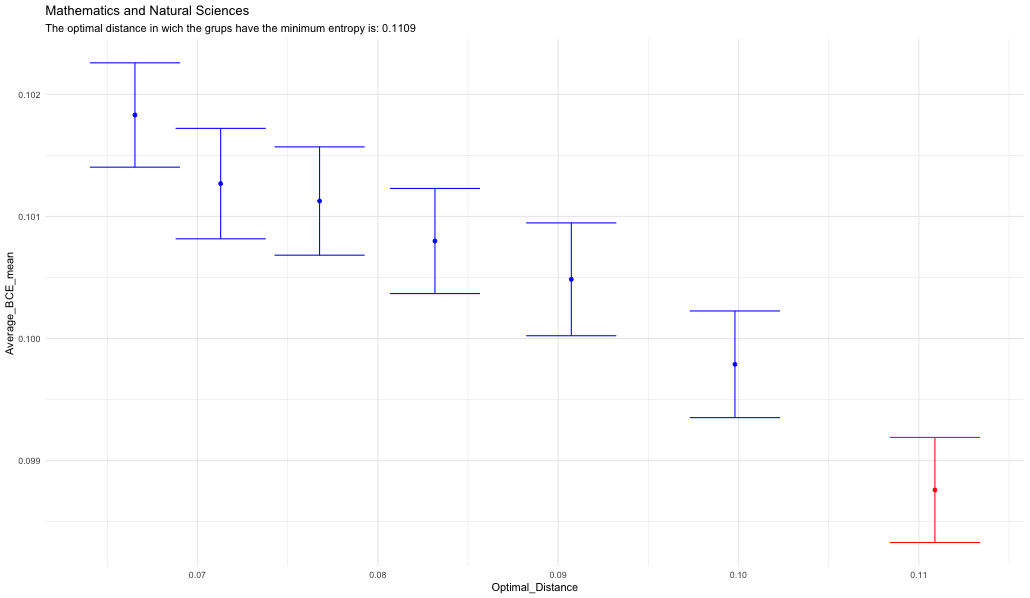
\includegraphics[width=0.8\textwidth]{Graph/Results/optimal_distance_bs30_MATHEMATICS_NATURAL_SCIENCES.png}
    \caption{Optimal Distance for Mathematics and Natural Sciences Majors}
    \label{fig:optimal_distance_math_natural_sci}
\end{figure}

\textbf{ 9. Medicine Majors}:
   As depicted in Figure \ref{fig:optimal_distance_medicine}, the optimal distance that minimizes the entropy in schooling decisions regarding the selection of Medicine majors is 0.1109.

\begin{figure}[htbp]
    \centering
    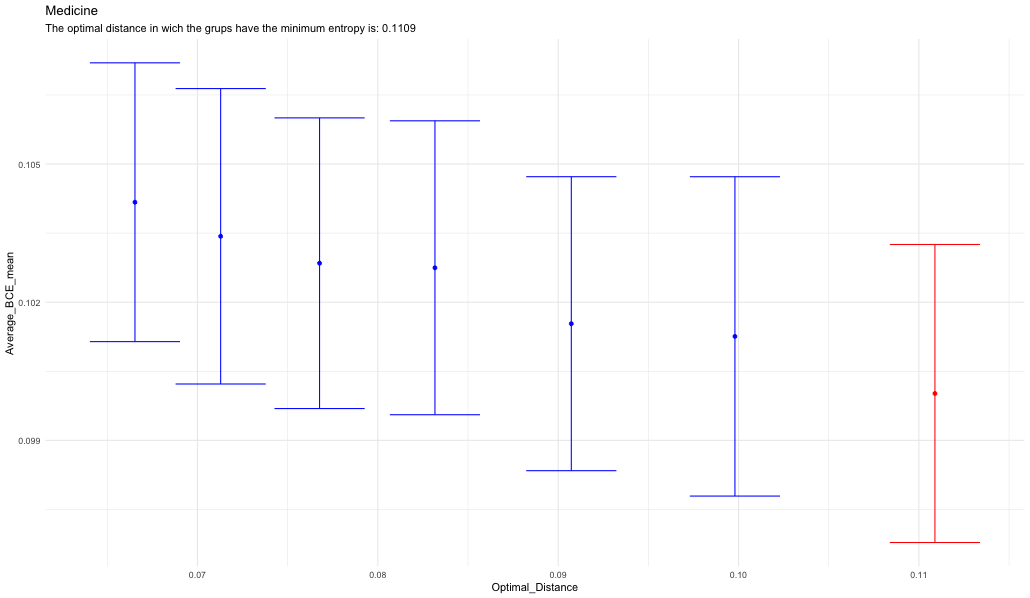
\includegraphics[width=0.8\textwidth]{Graph/Results/optimal_distance_bs30_MEDICINE.png}
    \caption{Optimal Distance for Medicine Majors}
    \label{fig:optimal_distance_medicine}
\end{figure}

\textbf{ 10. No Studies}:
    Figure \ref{fig:optimal_distance_no_studies} presents the optimal distance of 0.0832 for minimizing entropy in schooling decisions concerning not pursuing further studies.

\begin{figure}[H]
    \centering
    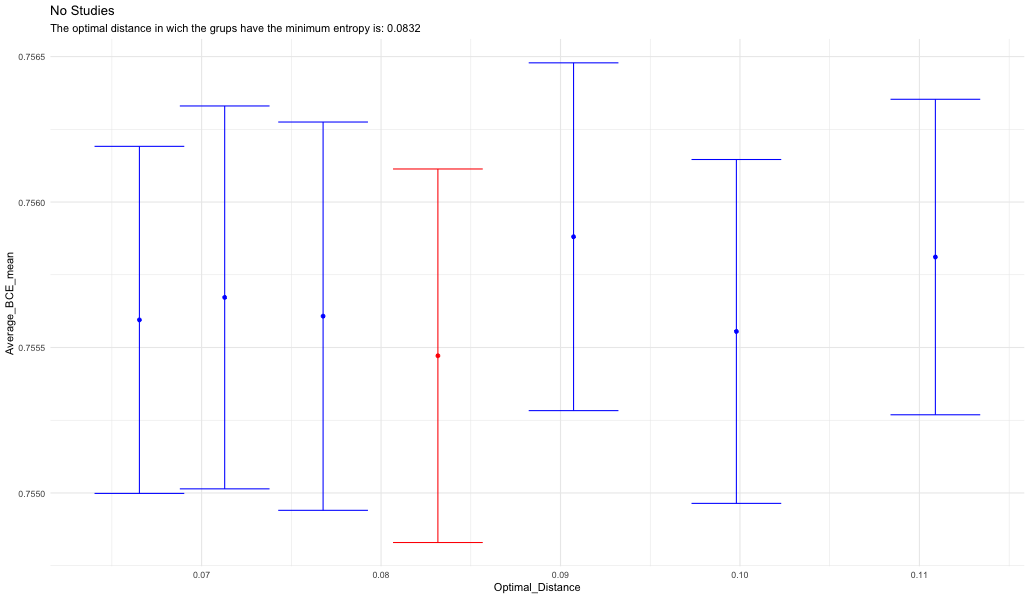
\includegraphics[width=0.8\textwidth]{Graph/Results/optimal_distance_bs30_NO_STUDIES.png}
    \caption{Optimal Distance for Not Pursuing Further Studies}
    \label{fig:optimal_distance_no_studies}
\end{figure}

\textbf{ 11. Social Sciences and Humanities Majors}:
    The optimal distance of 0.1109, as shown in Figure \ref{fig:optimal_distance_soc_sci_hum}, minimizes entropy in schooling decisions regarding Social Sciences and Humanities majors.

\begin{figure}[H]
    \centering
    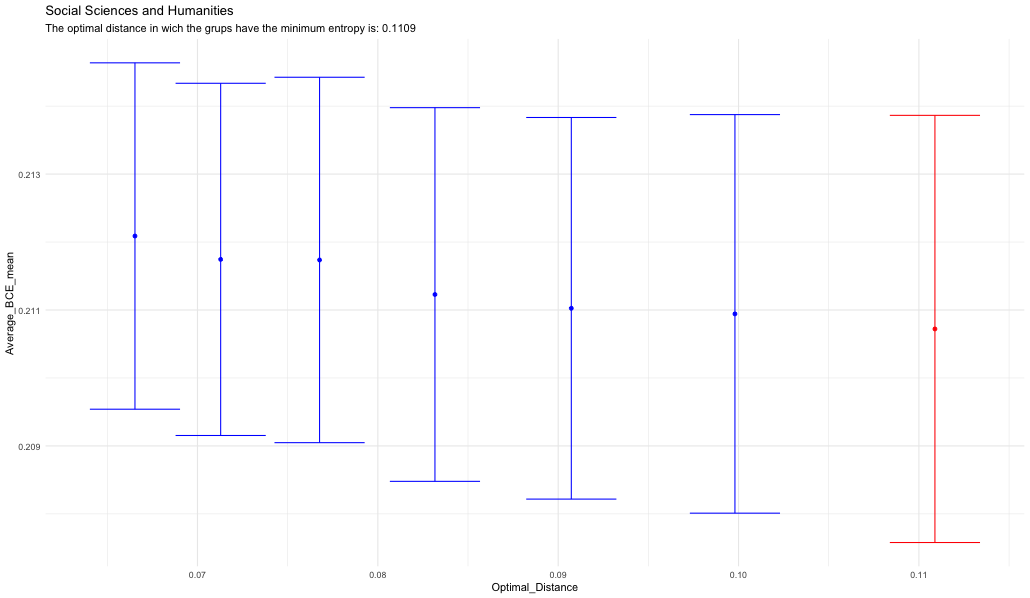
\includegraphics[width=0.8\textwidth]{Graph/Results/optimal_distance_bs30_SOCIAL_SCIENCES_HUMANITIES.png}
    \caption{Optimal Distance for Social Sciences and Humanities Majors}
    \label{fig:optimal_distance_soc_sci_hum}
\end{figure}
